This chapter intends to implement and analyse a controller ensuring safety if the demands from \autoref{req1}, \ref{req2} and \ref{req3} are obeyed. This shall first be tested on the slide movement on the Da Vinci surgical robot as it composes a prismatic joint and a 1:1 mapping from slide $joint\_angle$ to 1D position. Hence any inverse kinematic solver can be bypassed in the early phase of this project which is an important simplification to eliminate initial complications.

The slide movement is visualized in \autoref{fig:slidefig} and an overview of terms used in this section is found in \autoref{fig:safe:overview}. \Autoref{fig:safe:overview} encompasses likewise the case study considered in this chapter. It put forth the demands that the upper region, i.e. the interval $[\Lambda_{h+}:\Lambda_\text{lim+}]$ is an unsafe area and the rest is considered safe. Furthermore, everything outside the slide physical limits, i.e. $[-\infty:\Lambda_\text{lim-}]$ and $[\Lambda_\text{lim+}:\infty]$ is also considered unsafe. This case study is purely made up with the purpose to demonstrate the use of a safety controller.
\begin{figure}[H]
    \centering
    \begin{minipage}{.5\textwidth}
        \centering
        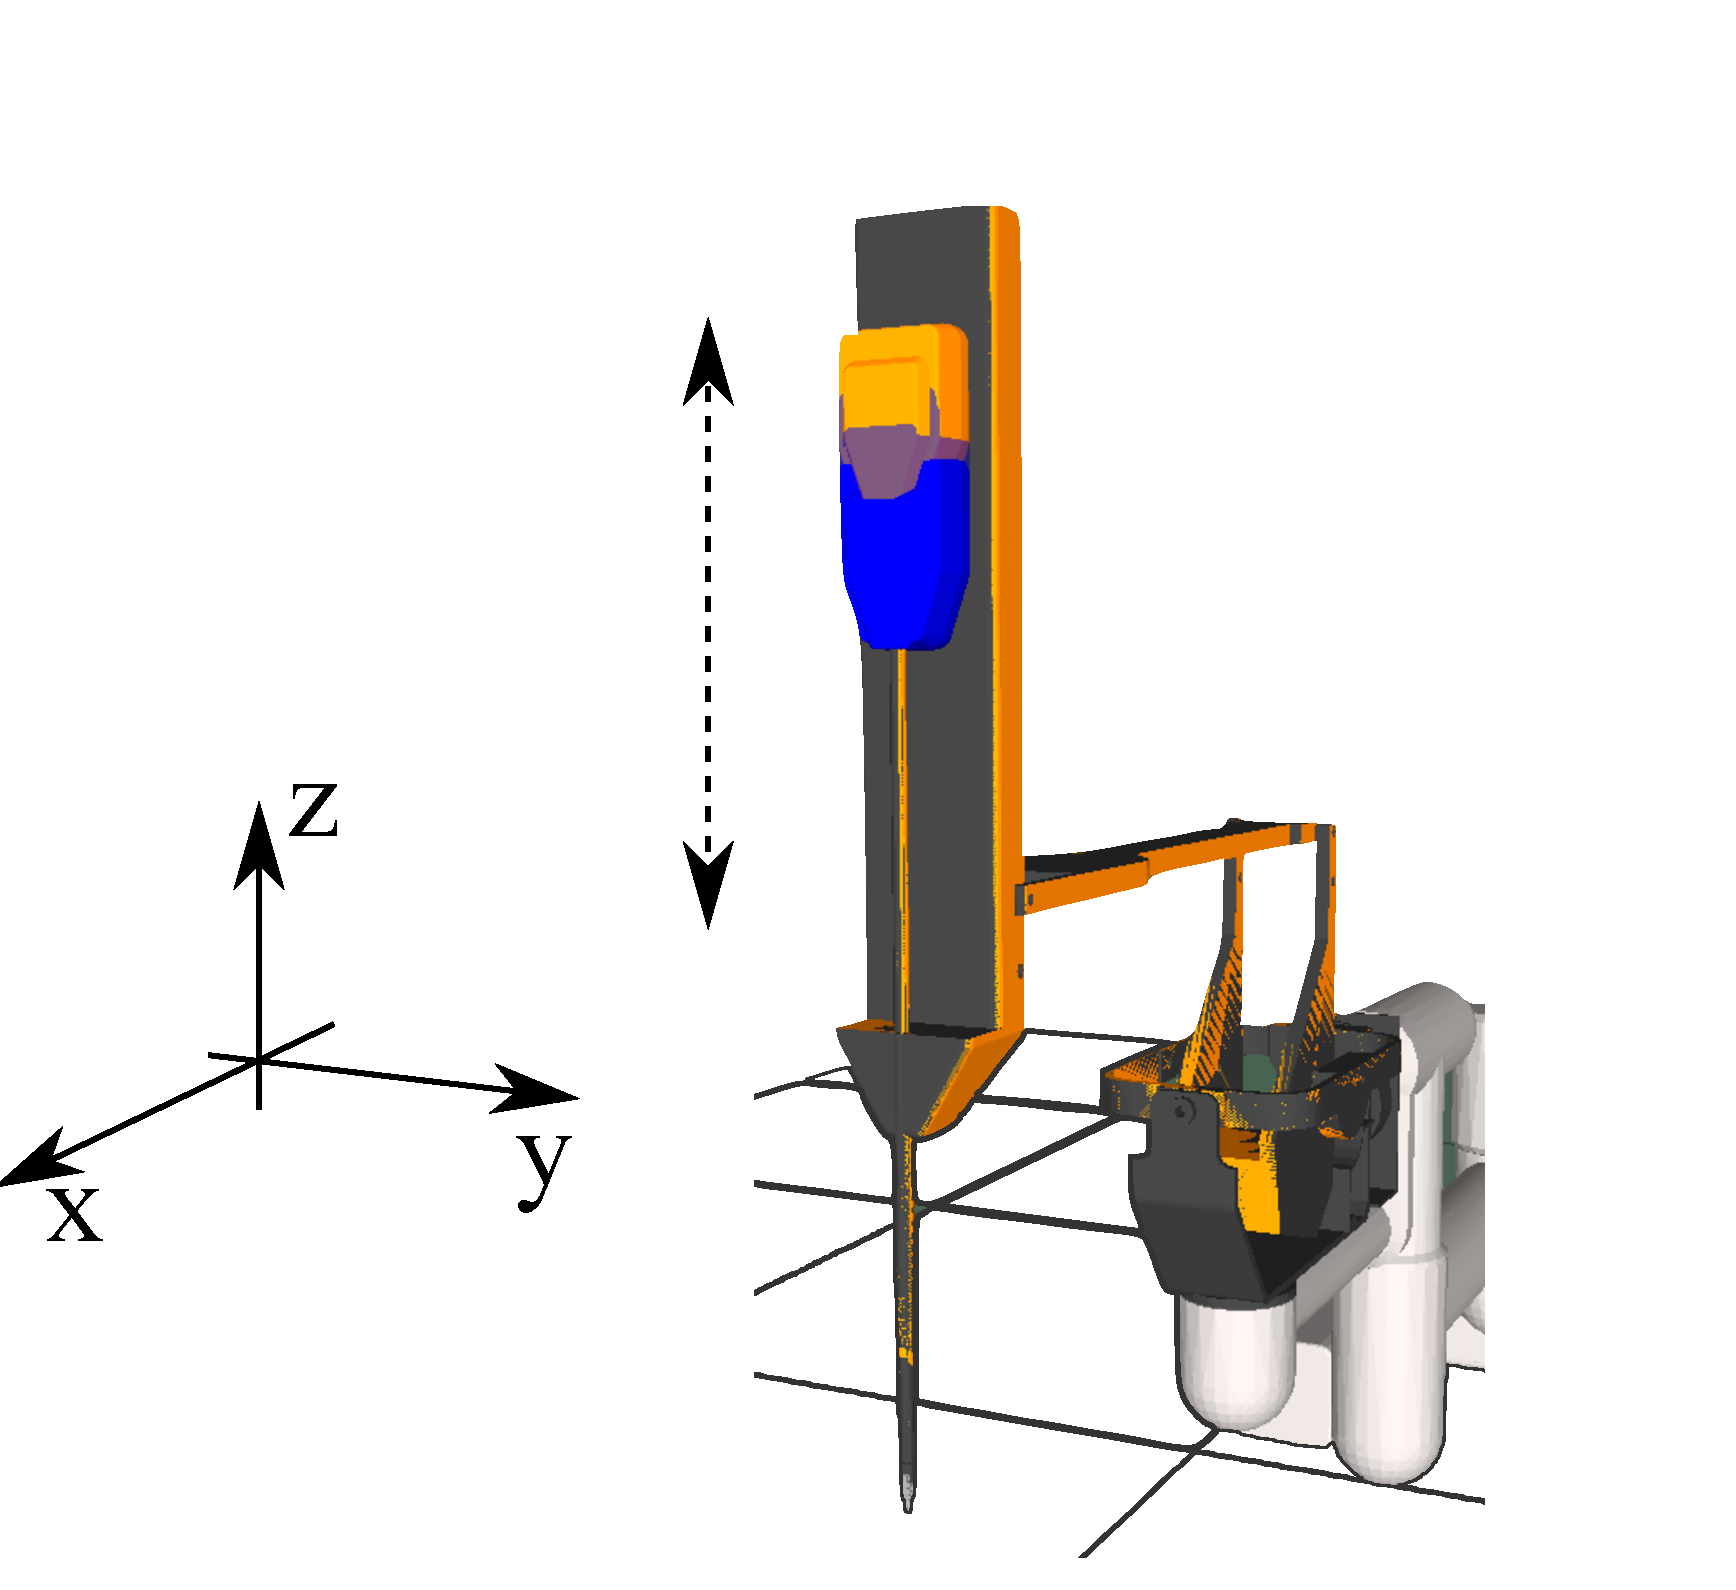
\includegraphics[width=0.84\linewidth]{slidemovefigure.pdf}
        \caption{Illustration of slide movement.}
        \label{fig:slidefig}
    \end{minipage}%
    \begin{minipage}{0.5\textwidth}
        \centering
        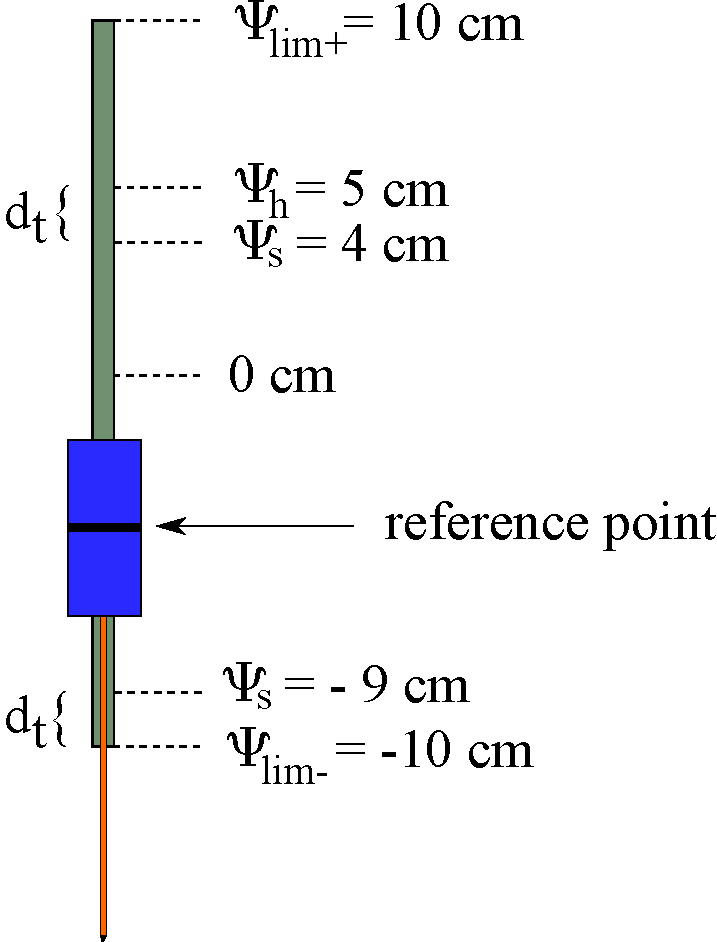
\includegraphics[width=0.8\linewidth]{slide_overview.pdf}
        \caption{Boundaries used in this section.}
        \label{fig:safe:overview}
    \end{minipage}
\end{figure}
The boundaries for the slide position are summed up in \autoref{tab:intervals}.
\begin{table}[H]
	\begin{tabularx}{\textwidth}{X X X }
\rowcolor{HeaderBlue} 
$\mathcal{X}$ & $\mathcal{X}_u$  & $\mathcal{X}_0$ \\
$x \in \{[\Lambda_{\text{lim}-},\Lambda_{s-}],[\Lambda_{s+},\Lambda_{\text{lim}+}]\}$  & $x \in \{[\Lambda_{\text{lim}-},\Lambda_{h-}],[\Lambda_{h+},\Lambda_{\text{lim}+}]\} $ & $x \in \{[\Lambda_{h-},\Lambda_{s-}],[\Lambda_{s+},\Lambda_{h+}]\}$  \\
\end{tabularx}
\caption{Global state intervals for the position where: $\Lambda_\text{lim}$ is the physical slide limit ($\pm$0.1\,m), $\Lambda_s$ is a soft limit denoting a transition line and $\Lambda_h$ is a hard limit where a trajectory at all cost can not cross. The interval $x \in [\Lambda_{s-},\Lambda_{s+}] \in \mathcal{Y}$ is safe thus $\tilde{u}(x)$ stated in \autoref{eq:utilde} can be used in this region.}
\label{tab:intervals}
\end{table}
As the control law stated in \autoref{eq:control_law} utilizes Lie derivatives, a system model is required before any controller design may be initiated.
%\hspace{1cm }\texttt{rostopic echo joint\_states/position[6]} \hspace{0.2cm} {\color{blue}{\# Be sure to have the ROS environment correctly configured according to \autoref{app:ros}}}
\section{Modelling of Slide Movement}\label{sec:model_slide}
To obtain a model of the slide movement, the step response will be measured.  This can be done by subscribing to the \texttt{joint\_state} topic in \gls{ros}. The experiment is described in further details in \autoref{app:meas}. The result is plotted in \autoref{fig:stepresponseslide}. 
\begin{figure}[H]
\center
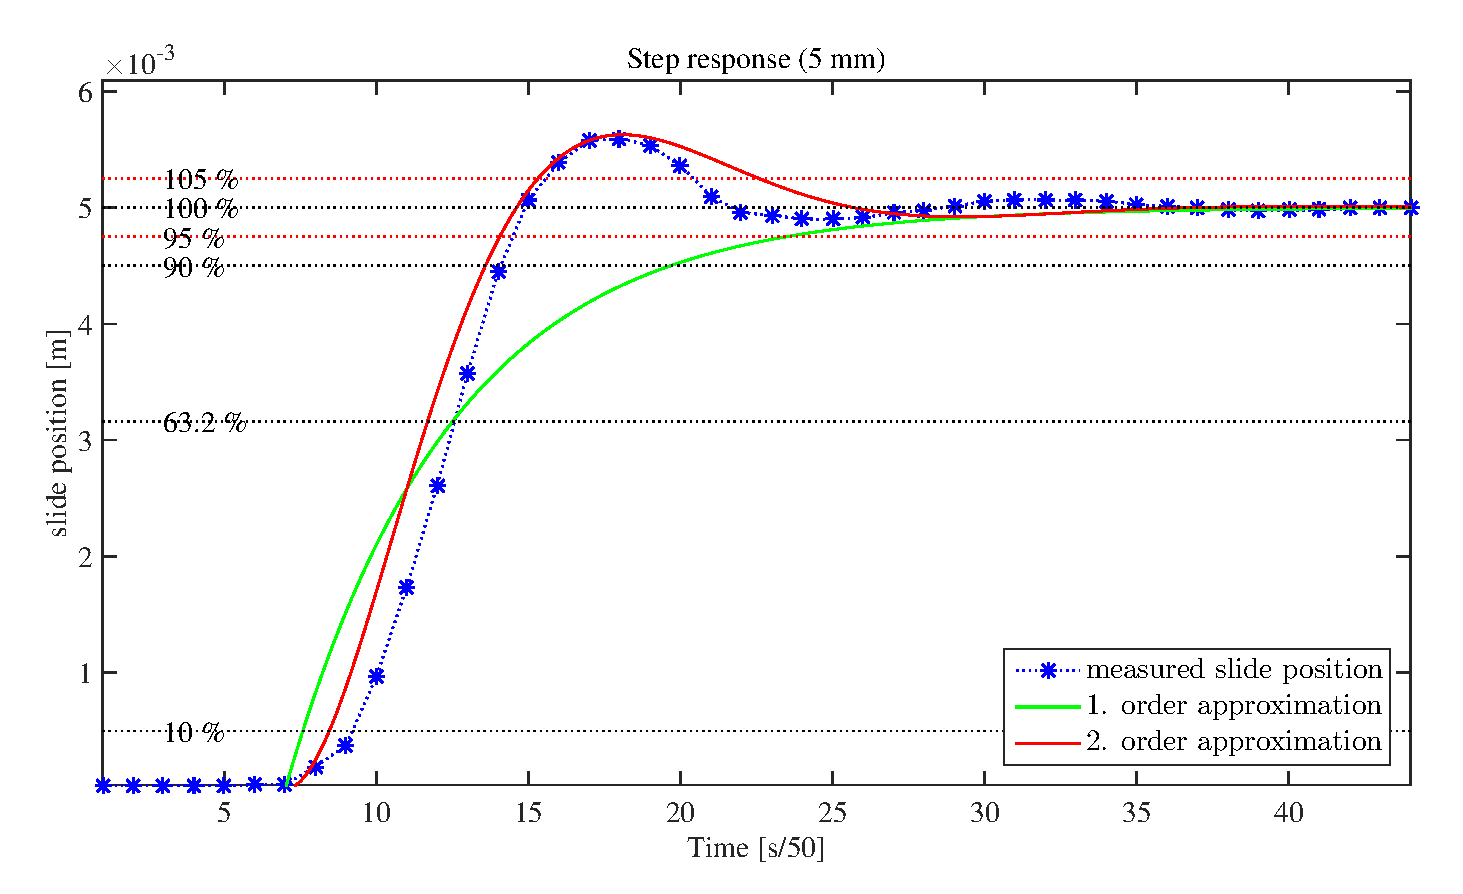
\includegraphics[scale=0.5]{step_slide.eps}
\caption{Step response from 0\,mm to 5\,mm. Plot details and measurements can be found in \autoref{app:cd} as \texttt{matlab\_scripts/slide\_step/plot\_slide\_pos.m}. The experiment is described in \autoref{app:meas}.}
\label{fig:stepresponseslide}
\end{figure}
The system can clearly be approximated with an underdamped second order model, however, for initial simplicity, merely a simple first order model of the slide movement is used. It shall, however, also be approximated as a second order system. This introduces a number of other challenges which is the reason for initial simplicity. These models will throughout this chapter be referenced as:
\begin{itemize}
\item One dimensional (1D) slide movement along the $z-$axis based on \underline{position} only, hence a first order system model.
\item One dimensional (1D) slide movement along the $z-$axis based on \underline{position and velocity}, hence a second order system model.
\end{itemize}
A first order approximation will be conducted first. 
\subsection{1D Model based on Position}\label{subsec:model_1d}
The system can be approximated to a linear first order system with a dominating time constant \gls{taus}. The time constant is read from \autoref{fig:stepresponseslide}:
\begin{flalign*}
\tau_s = 110\, \text{ms}
\end{flalign*} 
A linear system can be outlined as:
\begin{flalign}
& Y(s) = \dfrac{1}{\tau_s s + 1}U(s) =  \dfrac{1/\tau_s}{s + 1/\tau_s}\,U(s) = (s+1/\tau_s)^{-1}\,1/\tau_s\,U(s) \kk  \overset{\overset{Y(s)=(C(sI-A)^{-1}B+D)U(s)}{\longrightarrow}}{\scriptsize \text{compare to obtain SS form}}  \nonumber\\ 
& \dot{x} = \underbrace{-\tau_s^{-1}\,x}_{Ax} + \underbrace{\tau_s^{-1}}_{B} u
\label{eq:1storder_1D_ss}
\end{flalign}
The system matrix $A$ and the input matrix $B$ can be read from the above equation:
\begin{flalign*}
A = - \tau_s^{-1} =  \kk \wedge \kk B = \tau_s^{-1} \kk \wedge \kk C = 1 \kk \wedge \kk D = 0
\end{flalign*}
Which completes the first order approximation.

\subsection{1D Model based on Position and Velocity}\label{subsec:model_2d}
The second order approximation is based on the form:
\begin{flalign}
\dfrac{Y(s)}{U(s)} = \dfrac{\omega_n^2}{s^2 + 2\zeta \omega_n s + \omega_n^2}
\label{eq:2order}
\end{flalign}\\
\vspace{-0.6cm}
\begin{longtable}{p{.9\textwidth} p{.1\textwidth} p{.1\textwidth}} 
Where  & & \\
$Y(s)$ is the output in the Laplace domain  & [m] \\
$U(s)$ is the input in the Laplace domain  & [m] \\
\gls{omegan} is the natural frequency of the system & [rad/s] \\
\gls{zeta} is the damping coefficient  & [$\cdot$] \\
$s$ is the Laplace operator  & [rad/s] 
\end{longtable}
\vspace*{-0.2cm}
The model can unambiguous be approximated from the rise time $t_r$, settling time $t_s$ (5\,\% settling time) and the overshoot $M_p$ \citep{bib:dynamicsystems}. They are measured (conservatively) with the purpose to find $\omega_n$ and $\zeta$:
\begin{flalign*}
\omega_n = \dfrac{1.8}{t_r} = \dfrac{1.8}{0.106\,\text{s}} = 17 \,\text{rad/s} \kk \wedge \kk  \zeta = \dfrac{-1}{\omega_n \cdot t_s}\log (0.05) = \dfrac{-1}{17 \cdot 0.320}\log(0.05) = 0.55
\end{flalign*}
\Autoref{eq:2order} can be transferred to state space form: 
\begin{subequations}
\begin{flalign}
&Y(s)s^2 + 2\zeta \omega_n Y(s) s + \omega_n^2 Y(s) - \omega_n^2 U(s)  = 0 \\
&\ddot{y}(t) + 2\zeta \omega_n \dot{y}(t) + \omega_n^2 y(t) - \omega_n^2 u(t) = 0 \\
&\text{choose $y(t) = x_1(t) = \text{position} \kk \Rightarrow \kk \dot{x}_1(t) = x_2(t)$} \nonumber\\
&\begin{bmatrix}
\dot{x}_1(t)\\\dot{x}_2(t)
\end{bmatrix} = \begin{bmatrix}
0 & 1\\
-\omega_n^2  & -2\zeta \omega_n  
\end{bmatrix}\begin{bmatrix}
x_1(t) \\ x_2(t)
\end{bmatrix} + \begin{bmatrix}
0\\\omega_n^2
\end{bmatrix}u(t) \label{eq:2ndorder_1D_ss}\\
&\hspace{0.65cm}y(t) = \begin{bmatrix}
1 & 0
\end{bmatrix}\begin{bmatrix}
x_1(t) \\ x_2(t)
\end{bmatrix}
\end{flalign}
\end{subequations}
\vspace{-0.6cm}
\begin{longtable}{p{.8\textwidth} p{.1\textwidth} p{.1\textwidth}} 
Where  & & \\
$x_1(t)$ is the position& [m] \\
$x_2(t) = \dot{x}_1(t)$ is the velocity  & [m/s] \\
$y(t)$ is the output (slide position)  & [m] \\
$u(t)$ is the control input  & [$\cdot$]
\end{longtable}
\vspace*{-0.2cm}
Thus the linear system matrices can be outlined as:
\begin{flalign*}
A = \begin{bmatrix}
0 & 1\\
 -\omega_n^2   & -2\zeta \omega_n 
\end{bmatrix} \kk \wedge \kk B = \begin{bmatrix}
0 \\ \omega_n^2
\end{bmatrix} \kk \wedge \kk C = \begin{bmatrix}
1 & 0
\end{bmatrix} \kk \wedge \kk D = 0
\end{flalign*}
Which completes the second order model.

\section{Construction of CBF}\label{sec:construct_cbf}
To illustrate the usefulness of \glspl{cbf}, a palpable example hereof will be created with direct application to the Da Vinci robot. This example does not directly constitute application to a patient but favour the theory in a neat and comprehensible sense and secure a way to visually and physically verify the method.
%
%Consider the state intervals defined in \autoref{tab:intervals}.
%
%
\subsection{Construction of CBF based on First Order Model}\label{subsec:cbf-1order}
In this subsection, the state vector $x \in \mathbb{R}$ consist of the position only. Thus, a parabola is now introduced as \gls{cbf} as it allows an easy way to define $\mathcal{X}_u$ and $\mathcal{X}_0$ from \autoref{tab:intervals}. %A coordinate shift is performed such that the slide movement occurs along the $x$-axis instead of the $z$-axis. 
\begin{flalign}
B(x) &= ax^2+bx+c \label{eq:cbf1} 
\end{flalign}
This choice implies the $L_fB(x)$ shown below:
\begin{flalign}
L_fB(x) = \dfrac{d}{dx}B(x)f(x)\Bigm|_{f(x)=Ax}  = (2ax+b)(-\tau^{-1}x) = -2\tau^{-1}ax^2-\tau^{-1}bx \nonumber
\end{flalign}
\Autoref{req2} put forth the demand that $L_fB(x)<0$ when $L_gB(x) = 0$ as the input in that case will be insignificant. Ensuring that $L_gB(x) \neq 0 \in \mathcal{X}$ is therefore indeed sufficient. Analysis of $L_gB(x)$ shall reveal when $L_gB(x)=0$. Thus the equation below is analysed:
\begin{flalign*}
L_gB(x) \Bigm|_{g(x)=B} = ( 2ax + b ) \cdot \tau^{-1} = 0 \kk \Rightarrow \kk x = \dfrac{-b}{2a}
\end{flalign*}
Which indeed is the critical point for a one dimensional parabola. Thus if $L_fB(x) \leq 0 \,\,\, \forall \, x = \frac{-b}{2a}$ the \gls{cbf} is valid. Thereby, $L_fB(x) = 0$ is analysed:
\begin{flalign}
&L_fB(x) = 0 \kk \Leftrightarrow \kk  -2\tau^{-1}ax^2-\tau^{-1}bx = 0 \nonumber
 \\  &-2ax^2-bx = 0 \mm \Rightarrow \mm x = 
\begin{cases}
  \frac{-b}{2a} \\
   0   
\end{cases}
\label{eq:interval1}
\end{flalign}
Hence the \gls{cbf} is valid for all choices of $a,b$. The scalar $c$ must be less than zero to comply with \autoref{req3}.
At this point in time, three equations with three unknowns can be outlined to fulfil the initial demand in \autoref{fig:safe:overview}.
\begin{flalign*}
 \left.
 \begin{aligned}
a\,\Lambda_{h+}^2 + b\,\Lambda_{h+} + c = 0 \\
a\,\Lambda_{h-}^2 + b\,\Lambda_{h-} + c = 0 \\
a\left( \frac{\Lambda_{h-}+\Lambda_{h+}}{2}\right)^2 + b\left(\frac{\Lambda_{h-}+\Lambda_{h+}}{2}\right) + c = \underbrace{-0.025}_\text{any constant $<0$} 
\end{aligned}
\mm \right\}
 \qquad \begin{matrix}
 a &= \,\,\,\,\,\,\,\,1.7778 \\ b &= \,\,\,\,\,\,\,\,0.0889 \\ c &= -0.0089
 \end{matrix}
\end{flalign*}
%The interval where $B(x)$ is invalid can thereby be found from \autoref{eq:interval}:
%\begin{flalign*}
%B(x) \hspace{0.15cm} \text{invalid:} \mm  x \in [-0.0250,0] \kk \text{if} \mm L_gB(x) = 0
%\end{flalign*}
%However, this is indifferent as $\{\mathcal{X} \,\bigcap\, [\Lambda_{s-},\Lambda_{s+}]  \} = \emptyset $. Thus the barrier function is a valid \gls{cbf}. It is plotted in \autoref{fig:barrierfunction}
The \gls{cbf} is plotted in \autoref{fig:barrierfunction} from where it is seen that the demands from \autoref{tab:intervals} is fulfilled.
\begin{figure}[H]
\center
	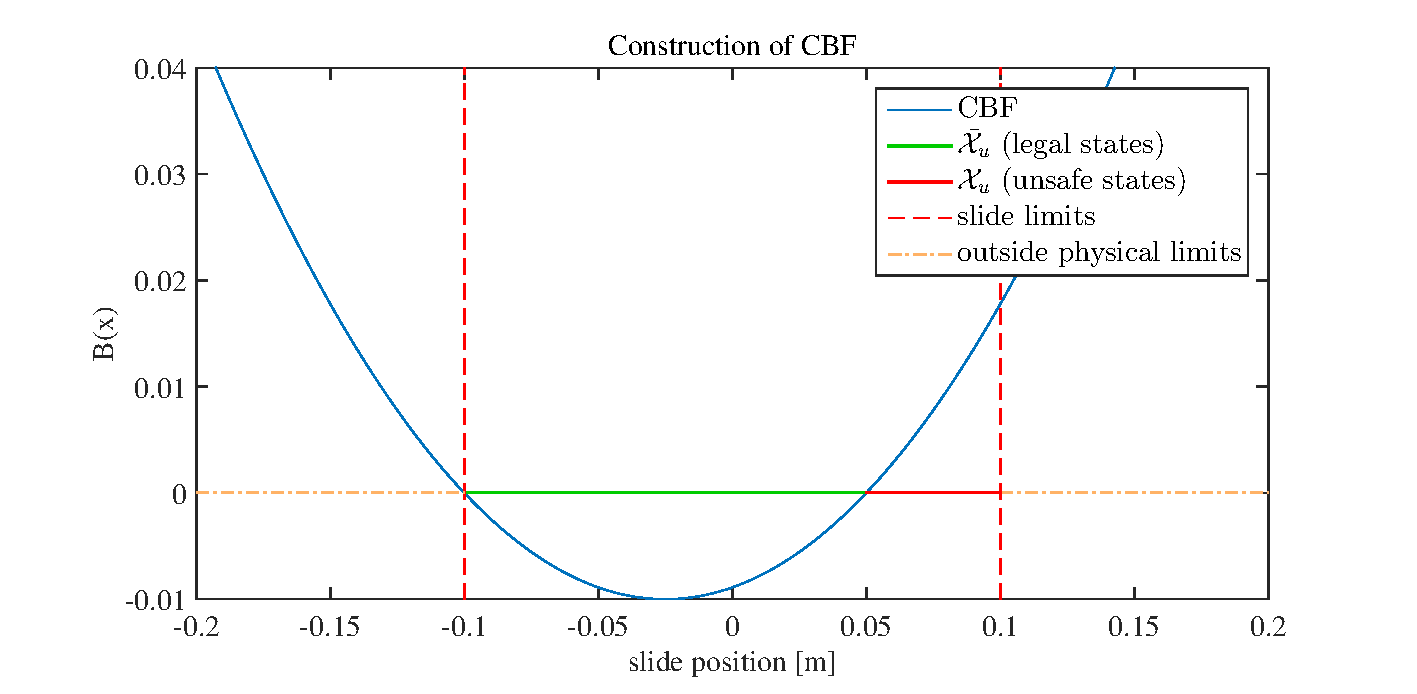
\includegraphics[scale=0.63]{parabel_1.eps}
	\caption{Barrier function along with the $\mathcal{X}_u$ and $\mathcal{X}_u^c$. Plot details and MATLAB script can be found in \autoref{app:cd} as \texttt{matlab\_scripts/plot\_parabola/plot\_parabola.m}}
	\label{fig:barrierfunction}
\end{figure}
\underline{Note:} The above analysis ensures safety regardless of $L_gB(x) = 0$ as it merely takes place at the critical point, i.e.:
\begin{flalign*}
 L_gB(x) = (2ax+b)B = 2ax\tau^{-1} + b\tau^{-1} = 0 \kk \Leftrightarrow \kk 2ax = -b \kk \Leftrightarrow \kk x = \dfrac{-b}{2a}
 \end{flalign*} 
 This is again the parabola extremity as it was found in \autoref{eq:interval1} and in fact an allowed exception for condition \autoref{req2} as the system is in its equilibrium.
\subsection{Construction of CBF Based on Second Order model}\label{subsec:cbf-2order}
Consider now $L_gB(x)$ for the same \gls{cbf} as given in \autoref{eq:cbf1}. Note that $B(x)$ is a function of position only, such that the CBF is:
\begin{flalign*}
B(x_1) = a\,x_1^2+ b\,x_1 + c
\end{flalign*}
Thus:
\begin{flalign*}
L_gB(x_1) = \dfrac{\partial B(x)}{\partial x}g(x) \Bigm|_{g(x)=B} =  
\begin{bmatrix}
\dfrac{\partial B(x)}{\partial x_1} & \dfrac{\partial B(x)}{\partial x_2} 
\end{bmatrix}\begin{bmatrix}
0 \\ \omega_n^2
\end{bmatrix} = 0 
\end{flalign*}
This put forth the requirement that $L_fB(x)<0\,\,\, \forall \, x$. Accordingly:
\begin{flalign}
L_fB(x) &= \dfrac{\partial B(x)}{\partial x}f(x) \Bigm|_{f(x)=Ax} = 
\begin{bmatrix}
\dfrac{\partial B(x)}{\partial x_1} & \dfrac{\partial B(x)}{\partial x_2} 
\end{bmatrix}
\begin{bmatrix}
1 & 0 \\
-2\zeta\omega_n & \omega_n^2
\end{bmatrix} \begin{bmatrix}
x_1 \\ x_2
\end{bmatrix} \nonumber \\
&= \dfrac{\partial B(x)}{\partial x_1} x_1 - \dfrac{\partial B(x)}{\partial x_2}2\zeta \omega_n x_1 - \dfrac{\partial B(x)}{\partial x_2} \omega_n^2 x_2 \nonumber \\
&= 2ax_1x_2 - x_2
\label{eq:2d_x1}
\end{flalign}
Note that the velocity appears in both terms. As the velocity can be both decreasing and increasing for all positions, this demand is impossible to fulfil with the chosen barrier function and therefore invalid. A solution may be to include the velocity in the barrier function. 

Consider the elliptic paraboloid as \gls{cbf}:
\begin{flalign}
B(x_1,x_2) =  \left( \dfrac{(x_1-x_{10})^2}{a_2^2} + \dfrac{(x_2-x_{20})^2}{b_2^2} \right) c_1 + c_2
\label{eq:cbf2}
\end{flalign}
\vspace{-0.6cm}
\begin{longtable}{p{.9\textwidth} p{.1\textwidth} p{.1\textwidth}} 
Where  & & \\
$x_1$ is the position  & [m] \\
$x_2$ is the velocity & [m/s] \\
$x_{10}$ is the extremity point for $x_1$ and thereby equilibrium point for an upward paraboloid & [m] \\
$x_{20}$ is the extremity point for $x_2$ and thereby equilibrium point for an upward paraboloid & [m/s] \\
$a_2$ is a constant that dictate the level of curvature $x_1-B(\textbf{x})$ plane & [$\cdot$] \\
$b_2$ is a constant that dictate the level of curvature $x_2-B(\textbf{x})$ plane & [$\cdot$] \\
$c_1$ is a constant that dictate if the paraboloid points upward ($c_1>0$) or downward ($c_1 < 0$)& [$\cdot$]  \\
$c_2$ is a constant that dictate the offset in $B(\textbf{x})$ axis & [$\cdot$] 
\end{longtable}
\vspace*{-0.2cm}
The elliptic paraboloid allows constraints in both position and velocity. Safety constraints in velocity are not of any significant importance as such, but they are necessary for $L_gB(x_1,x_2)$ such that it can obtain values different than zero in oppose to \autoref{eq:2d_x1}. To ensure that the position demands from \autoref{tab:intervals} are still fulfilled and to ensure that the position demands are fulfilled for all possible velocities (constrained by the slide movements physical limits), the below values are chosen:
\begin{flalign*}
x_{10} &= \dfrac{\Lambda_{h-}+\Lambda_{h+}}{2} = -1/40 \\
\Lambda_{x2-} &= -4 \kk \text{denotion of the lowest value where $B(0,x_2)=0$} \\
\Lambda_{x2+} &= 4 \kk \text{denotion of the highest value where $B(0,x_2)=0$} 
\end{flalign*}
Note that $|\Lambda_{x2-}|=|\Lambda_{x2+}|$ to ensure velocity equilibrium in 0\,m/s and note that the velocity outermost points are determined far bigger than the robots physical limits to ensure $\mathcal{X}_0 \notin \mathcal{X}_u $. Six equations with six unknowns can be outlined with the below numerical values.
\begin{flalign*}
 \left.
 \begin{aligned}
 \dfrac{(\Lambda_{h+}-x_{10})^2}{a_2^2} c_1 + c_2 = 0 \\
 \dfrac{(\Lambda_{h-}-x_{10})^2}{a_2^2} c_1 + c_2 = 0 \\
 \dfrac{\left(\frac{\Lambda_{h-}+\Lambda_{h+}}{2}-x_{10}\right)^2}{a_2^2} c_1 + c_2 = 0  = \underbrace{-1.000}_\text{any constant $<0$} \\
  \dfrac{(4-x_{20})^2}{b_2^2} c_1 + c_2 = 0 \\
 \dfrac{(-4-x_{20})^2}{b_2^2} c_1 + c_2 = 0 \\
 \dfrac{\left(0-x_{20}\right)^2}{b_2^2} c_1 + c_2 = -1  = \underbrace{-1.000}_\text{any constant $<0$}  
\end{aligned}
\mm \right\}
 \qquad \begin{matrix}
 x_{10} &= \,\,\,\,\,\,\,\,1/40 \\ x_{20} &= \,\,\,\,\,\,\,\,0.000 \\ a_2 &= \,\,\,\,\,\,\,\,3/40 \\ b_2 &=\,\,\,\,\,\,\,\,\,\,\, 4.000 \\
 c_1 &= \,\,\,\,\,\,\,\,1.000 \\ c_2 &= \,\,\,\,\,\,\,\, -1.000
 \end{matrix}
\end{flalign*}
The Lie derivatives can now be calculated as:
\begin{flalign}
L_gB(x_1,x_2) &= \dfrac{\partial B(x_1,x_2)}{\partial x} \cdot \textbf{B} = \begin{bmatrix}
\dfrac{\partial B(x_1,x_2)}{\partial x_1} & \dfrac{\partial B(x_1,x_2)}{\partial x_1}
\end{bmatrix}  \begin{bmatrix}
0 \\ \omega_n^2
\end{bmatrix} \\
 &= \begin{bmatrix}
 \dfrac{c_1(2x_1 + 2x_{10})}{a_2^2} &  \dfrac{c_1(2x_2 + 2x_{20})}{b_2^2}
\end{bmatrix}  \begin{bmatrix}
0 \\ \omega_n^2
\end{bmatrix} = 
\dfrac{c_1\omega_n^2(2x_2+2x_{20})}{b_2^2} \Bigm|_{x_{20}=0} \\
&= x_2\dfrac{2c_1\omega_n^2}{b_2^2}
\label{eq:LgB_2}
\end{flalign}
It is seen that $L_gB(x_1,x_2) \neq 0 \mm \forall \,\,\, x_2 \neq 0$. $L_fB(x_1,x_2)$ is for that reason analysed:
\begin{flalign}
L_fB(x_1,x_2) &= 
\dfrac{\partial B(x_1,x_2)}{\partial x} f(x)\Big|_{f(x) = \textbf{Ax}} = \begin{bmatrix}
\dfrac{\partial B(x_1,x_2)}{\partial x_1} & \dfrac{\partial B(x_1,x_2)}{\partial x_1}
\end{bmatrix} \begin{bmatrix}
0 & 1 \\
-\omega_n^2 & -2 \zeta \omega_n
\end{bmatrix} \begin{bmatrix}
x_1 \\ x_2
\end{bmatrix} \\
&= \begin{bmatrix}
 \dfrac{c(2x_1 + 2x_{10})}{a^2} &  \dfrac{c(2x_2 + 2x_{20})}{b^2}
\end{bmatrix} \begin{bmatrix}
x_2 \\ -\omega_n^2 x_1 - 2\zeta \omega_n x_2
\end{bmatrix} \\
&= \dfrac{c_1x_2(2x_1+2x_{10})}{a_2^2} - c_1(2x_2-2x_{20})\dfrac{(x_1\omega_n^2+2x_2\zeta \omega_n^2)}{b_2^2} \Big|_{x_{20} = 0} \\
&= x_2 \left( \dfrac{c_1(2x_1+2x_{10})}{a_2^2} - \dfrac{2c_1(x_1\omega_n^2+2x_2\zeta \omega_n^2)}{b_2^2} \right)
\label{eq:LfB_2}
\end{flalign}
It is noted that $L_fB(x_1,x_2) = 0 \mm \forall \,\,\, x_2 = 0$ which implies stability but not asymptotically stability. That is in general not good for physical systems and does neither fulfil \autoref{req2}. However, an engineering reflection and decision is taken at this point. Note that $x_2$ is nothing but the velocity and when $x_2 = 0$ the slide movement is steady. Thus $k_0(x)=0$ which indeed will force the slide movement to its origin as the control signal is the reference to a position controller. It implies hereafter $x_2 \neq 0$ again which is sufficient for the safety controller. %That is in this case a good thing as the slide will move back to the safe region and away from $\Lambda_{h-}$ and $\Lambda_{h+}$. Lastly, the velocity will never be truly zero due to the finite resolution, i.e. a finite sampling rate. For these reasons, the \gls{cbf} from \autoref{eq:cbf2} is accepted, well aware that the \gls{cbf} is insufficient,. It is, however, important to keep in mind that this is a dangerous decision. {\color{green}{RAFAL: Er det overhovedet OK at sige s\aa dan?}}

The elliptic paraboloid with its proper boundaries is plotted in \autoref{fig:barrierfunction_2d}.
\begin{figure}[H]
\center
	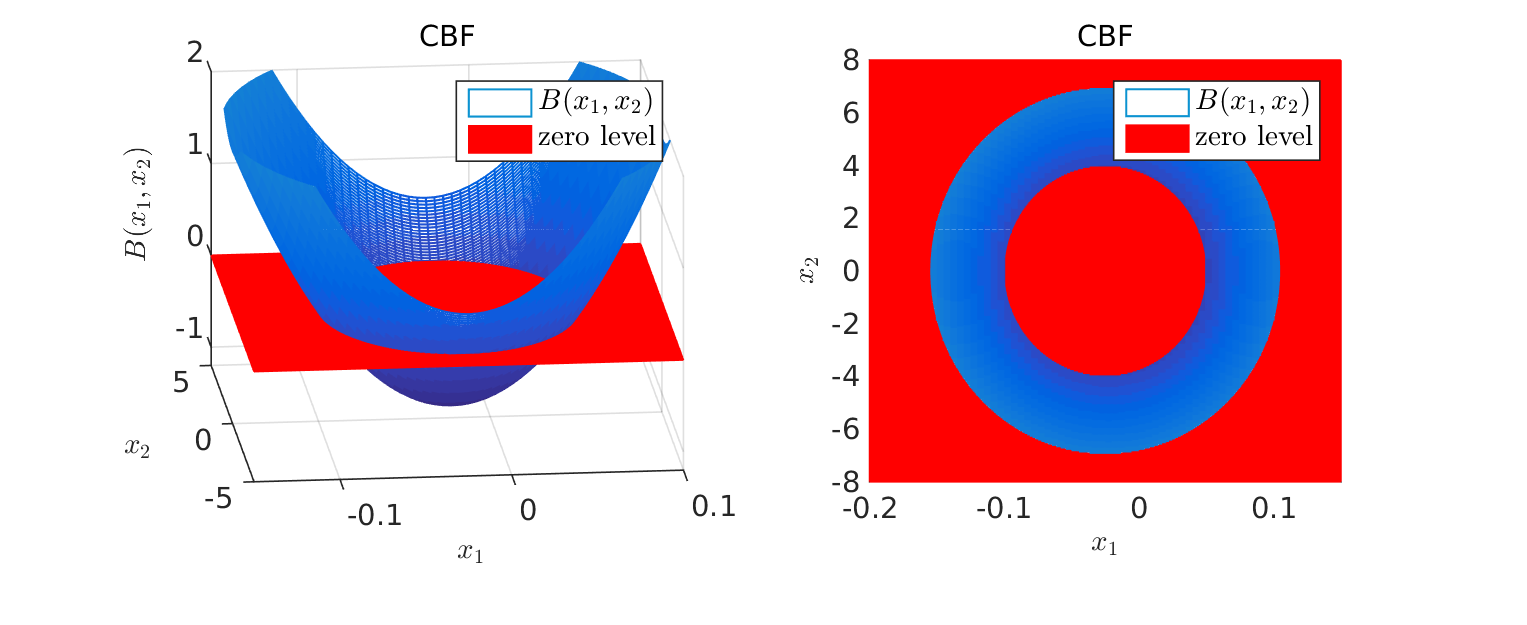
\includegraphics[scale=0.65]{cbf_2d.eps}
	\caption{CBF for the second order system model. Plot details and MATLAB script can be found in \autoref{app:cd} as \texttt{matlab\_scripts/plot\_cbf\_2d/plot\_cbf\_2d.m}}
	\label{fig:barrierfunction_2d}
\end{figure}
It is from \autoref{fig:barrierfunction_2d} seen how the specified regions, i.e. $x_2 \in [\Lambda_{x2-},\Lambda_{x2+}]$ and $x_1 \in [\Lambda_{h-},\Lambda_{h+}]$, both fulfils that $B(x_1,x_2)<0$ and thus everything else is unsafe, i.e. $B(x) > 0$. It is also seen that $x_2$ is approximately vertical in the boundaries of $x_1$ when the big numerical difference in the axes are taken into account.

\textbf{\underline{\textit{Remark:}}} The issue caused by $x_2=0$ is not only the case for this specific \gls{cbf} but for many \gls{cbf}s. Take for example another CBF that could fulfil the position requirements from \autoref{tab:intervals}:
\begin{flalign*}
B(x_1,x_2) = \cos (c_3 x_1 + c_4) \cdot \cos (c_5 x_2 + c_6)
\end{flalign*}
It turns out that the coefficients $c_3 = 21.00, c_4 = 119.91, c_5 = 0.50, c_6 = 3.15$ induce a CBF with the same properties as the one depicted in \autoref{fig:barrierfunction_2d}. The \gls{cbf} is outlined graphically in \autoref{fig:barrierfunction_example_sinus}.
\begin{figure}[H]
\center
	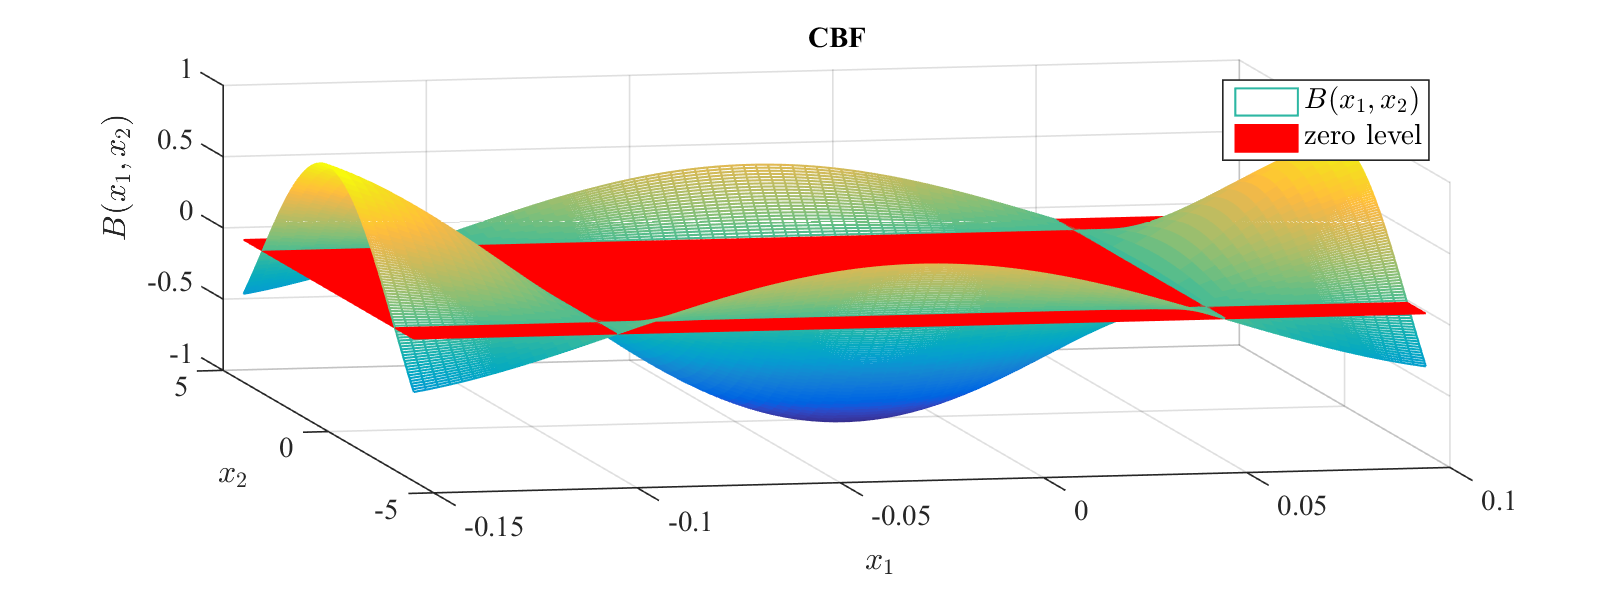
\includegraphics[scale=0.65]{cbf_example_sinus.eps}
	\caption{CBF. Example to demonstrate how other CBFs suffer when $x_2 = 0$.}
	\label{fig:barrierfunction_example_sinus}
\end{figure}
Thus $L_gB(x_1,x_2)$ can be found as:
\begin{flalign*}
L_gB(x_1,x_2) = -c_5 \omega_n^2 \cos (c_4-c_3 x_1)\sin(c_6 + c_5 x_2)
\end{flalign*}
Now note that when $c_6+c_5x_2 = \pi \,\, \Rightarrow \,\, L_gB(x_1,x_2) = 0$ such that $x_2 \approx 0$ implies the requirement that $L_fB(x_1,x_2) < 0 \,\,\, \forall \, x_2 \approx 0$. % As $L_gB(x_1,x_2) \neq 0 \,\, \forall \,\, x_2 \approx 0$, requirements for $L_fB(x_1,x_2)$ is necessary. 
However, taking a look at $L_fB(x_1,x_2)$:
\begin{flalign*}
L_fB(x_1,x_2) = 
c_5\cos (c_4 + c_3 x_1) \sin(c_6+c_5 x_2)(x_2 \omega_n^2 + 2 x_1 \zeta \omega_n) - c3 x_2 \cos(c_6 + c_5 x_2) \sin(c_4 + c_3 x_1)
\end{flalign*}
Quickly pose the fact that $L_fB(x_1,x_2 ) \nless 0 \,\, \forall \,\, x_2 \approx 0$ due to the sign alternation caused by the term $c_5\cos(c_4 + c_3 x_1)$ in the boundaries.

\subsection{Control Design based on First Order Model}\label{sec:K_Nbar_1D_1storder}
The be able to find $k_0(x)$ from \autoref{eq:control_for_safety}, the constant $\epsilon$ used in \autoref{eq:smoothness} must be found. It can be determined from the \gls{cbf} from \autoref{eq:cbf1} such that it complies with the requirements from \autoref{tab:intervals}:
\begin{flalign}
\epsilon = |B(\Lambda_{s+})| = |B(\Lambda_{s-})| = 0.00249
\label{eq:epsilon}
\end{flalign}
This is a need way to incorporate the transition between $\Lambda_s$ and $\Lambda_h$ because $k_0(x)$ kicks in slowly when the trajectory exceeds $\Lambda_s$. \Autoref{fig:epsilon_plot} illustrates how $\epsilon$ and $B(x)$ is connected.
\begin{figure}[H]
	\center
		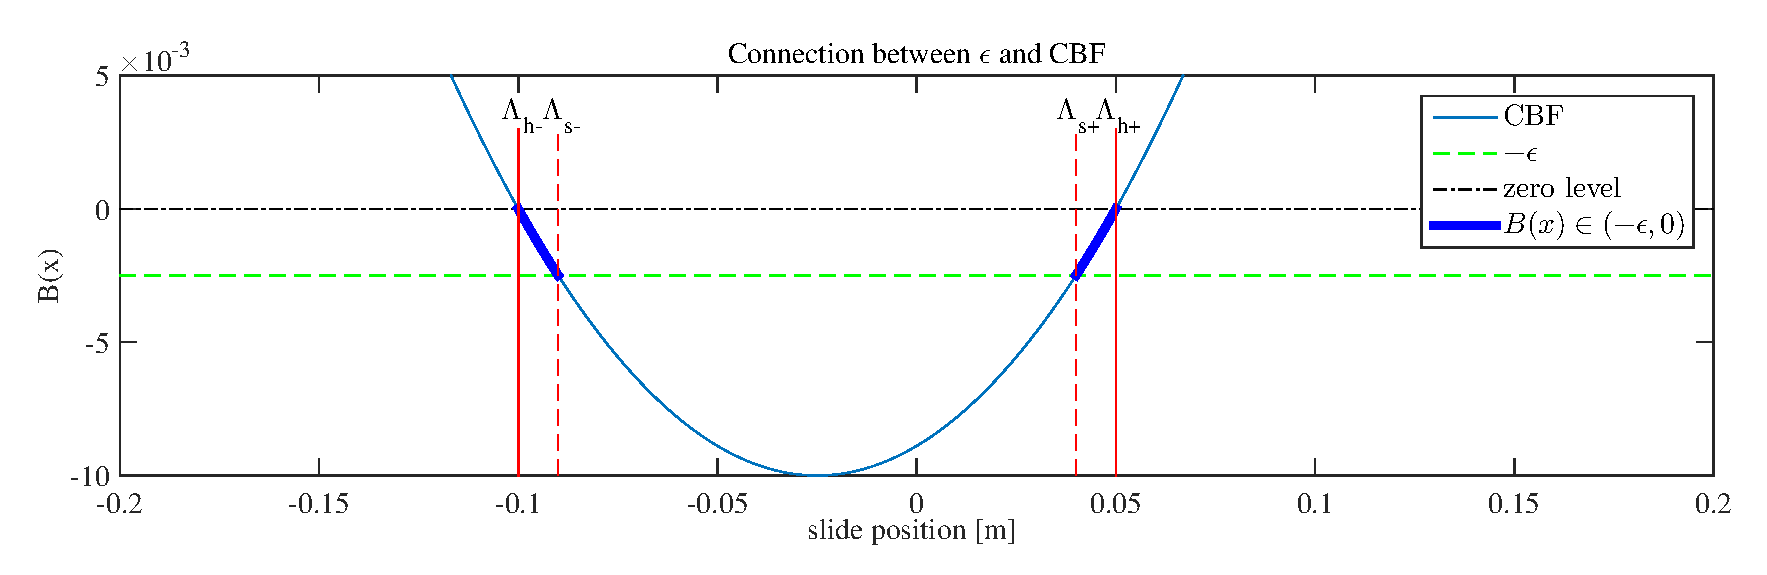
\includegraphics[scale=0.55]{epsilon_plot.eps}
	\caption{Connection between $\epsilon$ and CBF. MATLAB script and plot details can be found in \autoref{app:cd} as \texttt{matlab\_scripts/plot\_epsilon/plot\_epsilon\_slide\_1d.m}}
	\label{fig:epsilon_plot}
\end{figure}

The system is approximated to a linear system on the form $\dot{x}=Ax+Bu$, thus pole placement can be used. No constraints to the constant feedback matrix $K$ will be outlined except stability. It will therefore be determined from the pole placement method where a closed loop pole that is ten times faster than the open loop pole will be placed. Ackermann's formula can be used \citep{bib:acker}:
\begin{enumerate}
\item Identify the desired closed loop polynomial as $A_{cl}(s) = s^n + a_{c(n-1)}s^{n-1}  +  \cdots + a_ {c1}s + a_{c0}$: 
\begin{flalign*}
A_{cl}(s) = s + 10\,\tau^{-1}
\end{flalign*}
\item Identify the open loop polynomial as $A_{ol}(s) = s^n + a_{n-1}s^{n-1} +  \cdots + a_1s + a_0$: 
\begin{flalign*}
A_{ol}(s) = \lambda + \tau^{-1}
\end{flalign*}
\item Compute the feedback matrix in controllable canonical form:
\begin{flalign*}
 \bar{K}^T = \begin{bmatrix}   
 \bar{k_1} \\
 \vdots \\
 \bar{k_n}
 \end{bmatrix} = \begin{bmatrix}
 a_{c0} - a_0 \\
 \vdots \\
 a_{c(n-1)} - a_{n-1}
 \end{bmatrix} \kk \Rightarrow  \kk \bar{K}^T = 10\,\tau^{-1} - \tau^{-1} = 9\,\tau^{-1}
\end{flalign*}
\item Compute the similarity transform $Q$ recursively as:\\ 
\begin{minipage}[t]{0.3\textwidth}
\begin{flalign*}
&Q = \begin{bmatrix}
q_1 & q_2 & \cdots & q_n
\end{bmatrix} \\
&\text{where:}\\
&\kk q_n = B \\
&\kk q_{j-1} = A\,q_j + a_{j-1}B\\
{\color{white}{white}}\hspace{-0.5cm}
\end{flalign*}
\end{minipage}
\begin{minipage}[t]{0.1\textwidth}
\begin{flalign*}
\Rightarrow
\end{flalign*}
\end{minipage}
\begin{minipage}[t]{0.2\textwidth}
\begin{flalign*}
Q = \tau^{-1}
\end{flalign*}
\end{minipage}
\item Compute the feedback matrix as:
\begin{flalign}
K = \bar{K}\,Q^{-1} = 9\,\tau^{-1}\dfrac{1}{\tau^{-1}} = 9
\label{eq:K_1}
\end{flalign}
\end{enumerate}
The constant feedback matrix, $\bar{N}$, can be computed as \citep{bib:Nbar}:
\begin{flalign}
\bar{N} = - \left( C\,A_{cl}^{-1}\,B \right)^{-1} =  - \left( C\,(A-B\,K)^{-1}\,B \right)^{-1} = 10
\label{eq:barm_1}
\end{flalign}
%\subsubsection*{Merged Control Law}
With the Lie derivatives computed as:
\begin{flalign}
L_fB(x) = -2\tau^{-1}ax^2-\tau^{-1}bx \kk \wedge \kk L_gB(x) = 2ax\tau^{-1} + b\tau^{-1}
\label{eq:lies_1}
\end{flalign}
The complete control law can be determined from \autoref{eq:control_law}:
\begin{tcolorbox}
\begin{flalign*}
u(x) = \sigma(x)k_0(x)+(1-\sigma(x))(\bar{N} \cdot x_\text{ref}-Kx) 
\end{flalign*}
\vspace{-0.8cm}
\begin{longtable}{p{.9\textwidth} p{.1\textwidth} p{.1\textwidth}} 
Where  & & \\
$\sigma(x)$ is computed from \autoref{eq:smoothness} with the $\epsilon$ found in \autoref{eq:epsilon} and the \gls{cbf} found in \autoref{eq:cbf1} &  \\
$k_0(x)$ is computed from \autoref{eq:control_law} with the Lie derivatives states in \autoref{eq:lies_1} & \\
$\bar{N}$ is found in \autoref{eq:barm_1} & \\
$K$ is found in \autoref{eq:K_1} &
\end{longtable}
\vspace*{-0.2cm}
\end{tcolorbox}
This completes the control design based on a first order system approximation. 
\subsection{Control Design Based on a Second Order Model}\label{sec:K_Nbar_1D_2ndorder}
To design the smoothing in the transition area $\Delta_t$ for the second order approximation, the $\epsilon$ found in \autoref{eq:epsilon} is used again such that the \gls{cbf} from \autoref{eq:cbf1} is reused here, i.e $\sigma(x_1)$ from \autoref{eq:smoothness} is a function of position only. {\color{red}{Overvej om kriteriet skal v\ae re h\aa rdere??}}
\begin{flalign}
\sigma(x) = 
\begin{cases}
0 & \text{if} \mm B(x) \leq -\epsilon \\
-2  \left( \dfrac{B(x}{\epsilon} \right)^3 - 3\left( \dfrac{B(x_1)}{\epsilon} \right)^2 +1 \kk &\text{if} \mm B(x_1) \in (-\epsilon,0) \\
1  &\text{if} \mm B(x) \geq 0
\end{cases}
\end{flalign} 
\vspace{-0.8cm}
\begin{longtable}{p{.9\textwidth} p{.1\textwidth} p{.1\textwidth}} 
Where  & & \\
$B(x_1) = ax_1^2 + bx_1 + c$ as it is stated in \autoref{eq:cbf1} &
\end{longtable}
\vspace*{-0.2cm}
The design of $K$ and $\bar{N}$ will follow the exact same procedure as described for the first order model except now $K \in \mathbb{R}^{1 \times 2}$. $\bar{N}$ remains as a scalar. The entire design procedure is therefore not carried through again.  

However, it is of interest to slow down the system dynamics slightly compared to the controller based on a first order system. This is to enter the unsafe region with a lower velocity and thereby allow the safety controller some transition space to navigate the trajectory back to its safe area. The eigenvalues of the second order system is found to:
\begin{flalign*}
\lambda_\text{2nd order system} = \begin{cases}
-10.295 -14.765\,j \\
-10.295 +14.765\, j
\end{cases}
\end{flalign*}
The feedback vector can be found with the MATLAB command \texttt{acker} based on pole placement slightly faster than the system itself.
\begin{flalign}
K = \texttt{acker(A,B,C,D,[-40 -50])} = \begin{bmatrix}
5.173  &  0.214
\end{bmatrix}
\label{eq:K_2}
\end{flalign}
The DC gain can now be corrected with:
\begin{flalign}
\bar{N} = - \left( C\,A_{cl}^{-1}\,B \right)^{-1} =  - \left( C\,(A-B\,K)^{-1}\,B \right)^{-1} = 6.173
\label{eq:Nbar_2}
\end{flalign}
The complete controller is now designed as:
\begin{tcolorbox}
\begin{flalign*}
u(x) = \sigma(x)k_0(x)+(1-\sigma(x))(\bar{N} \cdot x_\text{ref}-Kx)
\end{flalign*}
\vspace{-0.8cm}
\begin{longtable}{p{.9\textwidth} p{.1\textwidth} p{.1\textwidth}} 
Where  & & \\
$\sigma(x)$ is computed from \autoref{eq:smoothness} with the $\epsilon$ found in \autoref{eq:epsilon} and the \gls{cbf} found in \autoref{eq:cbf1} &  \\
$k_0(x)$ is computed from \autoref{eq:control_law} with the Lie derivatives found in \autoref{eq:LgB_2} and \ref{eq:LfB_2} & \\
$\bar{N}$ is found in \autoref{eq:Nbar_2} & \\
$K$ is found in \autoref{eq:K_2} &
\end{longtable}
\vspace*{-0.2cm}
\end{tcolorbox}
This completes the control design. The implementation constitutes both a MATLAB simulation and an actual implementation on the Da Vinci robot in \gls{ros}. The MATLAB implementation is outlined first. 
\vspace{-0.3cm}
\section{MATLAB Results}\label{sec:matlab-results-slide-safety}
\vspace{-0.2cm}
The results shown in this section are based on the implemented controller found in \autoref{app:slide_implement_1} and in \autoref{app:cd} under the path \texttt{matlab\_scripts\_slide\_controller\_slide\_controller.m}. All plots are made with the following characteristics:
\begin{itemize}
\item The sampling rate is tested with both $f_s = 2\,$kHz (expected sampling rate in the long run) and $f_s = 100\,$Hz (current limitation of the sample rate caused by the TCP/IP communication channel).
\item The control signal is limited to $\pm 0.1$\,m (actual limit for slide movement).
\item The velocity is limited to $\pm$1\,m/s (actual limit for slide movement).
\item The forward euler method is used to extrapolate the states.
\item The design parameter $\kappa$ from \autoref{eq:control_law} is set to $\kappa=1$ (neutral).
\item The simulation time is 5\,s. Various setpoints ought to indicate the behaviour in different regions.
\end{itemize}
The \texttt{model} variable in line 7 in \autoref{app:slide_implement_1} is set to the number 1 for the first order model and 2 for the second order model. 
\vspace{-0.3cm}
\subsection{MATLAB Results based on First Order Model}\label{subsec:matlab-results-1order}
The state trajectory composing slide position is plotted in \autoref{fig:trajectory1}
\begin{figure}[H]
	\center
		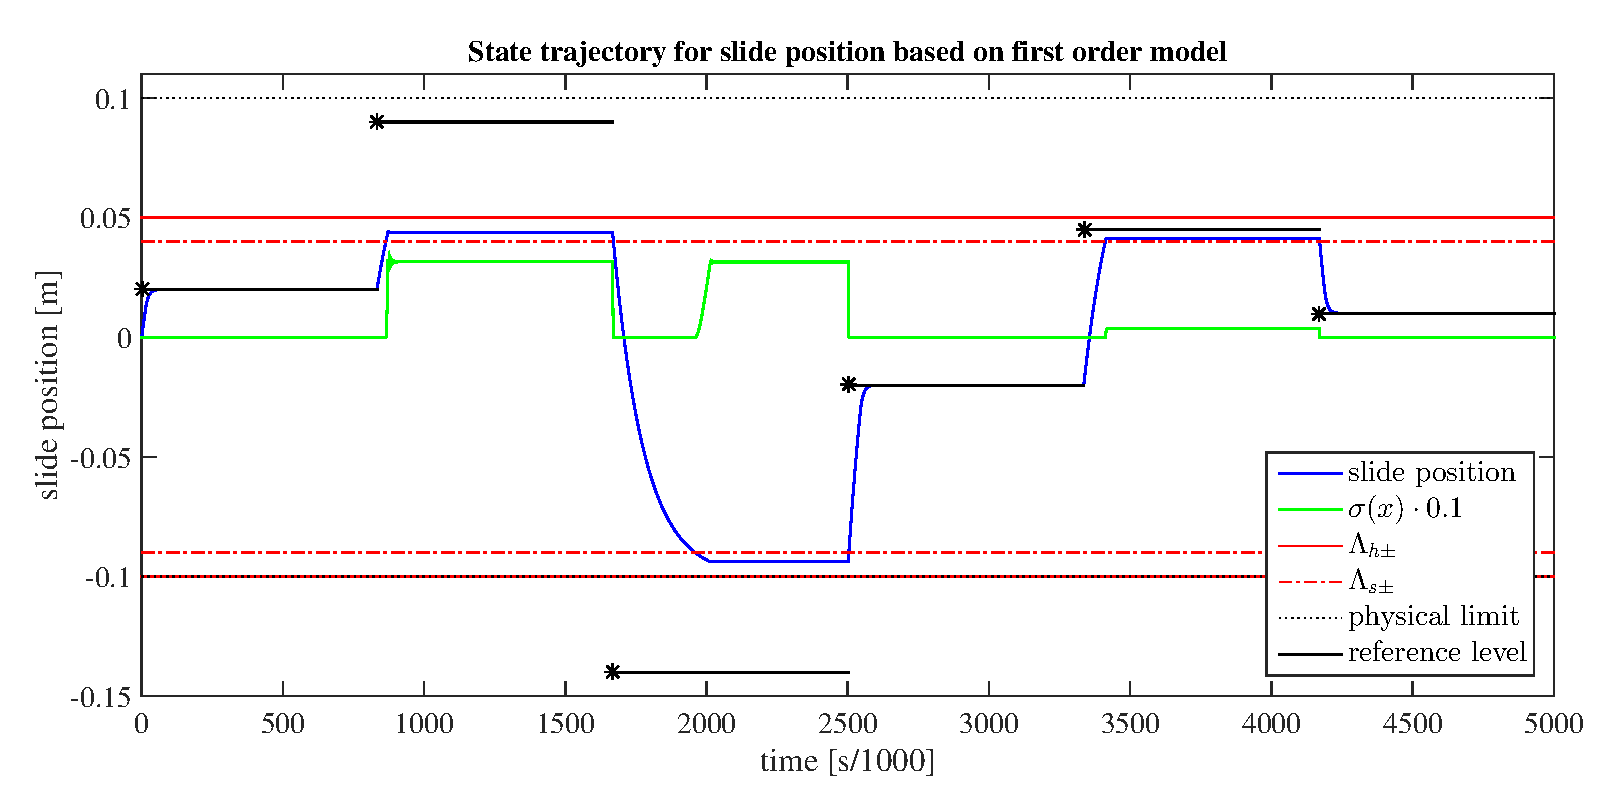
\includegraphics[scale=0.6]{trajectory_slide.eps}
	\caption{State trajectory for slide position for $\kappa=1$. MATLAB implementation can be found in \autoref{app:slide_implement_1}. The plot is based on forward euler with a sampling rate of $1\,$kHz. It is seen how the correct position is obtained in the interval $[\Lambda_{s-}:\Lambda_{s+}$]. When setpoints are given outside the safe area, the safety controller ensures that the hard boundaries $\Lambda_{h+}$ and $\Lambda_{h-}$ are not exceeded at any time and that the position finds its equilibrium at some arbitrary state.}
	\label{fig:trajectory1}
\end{figure}
Varying $\kappa$ increases the aggressivity of the safety controller and can create fluctuations in the transition area if the sampling rate is too low. Likewise $\sigma(x)$ will fluctuate along with an increased $\kappa$. One must be careful when increasing $\kappa$ when the sampling rate is relatively low. %The effect of increasing $\kappa$ ten times is shown in \autoref{fig:trajectory2}.
%\begin{figure}[H]
%	\center
%		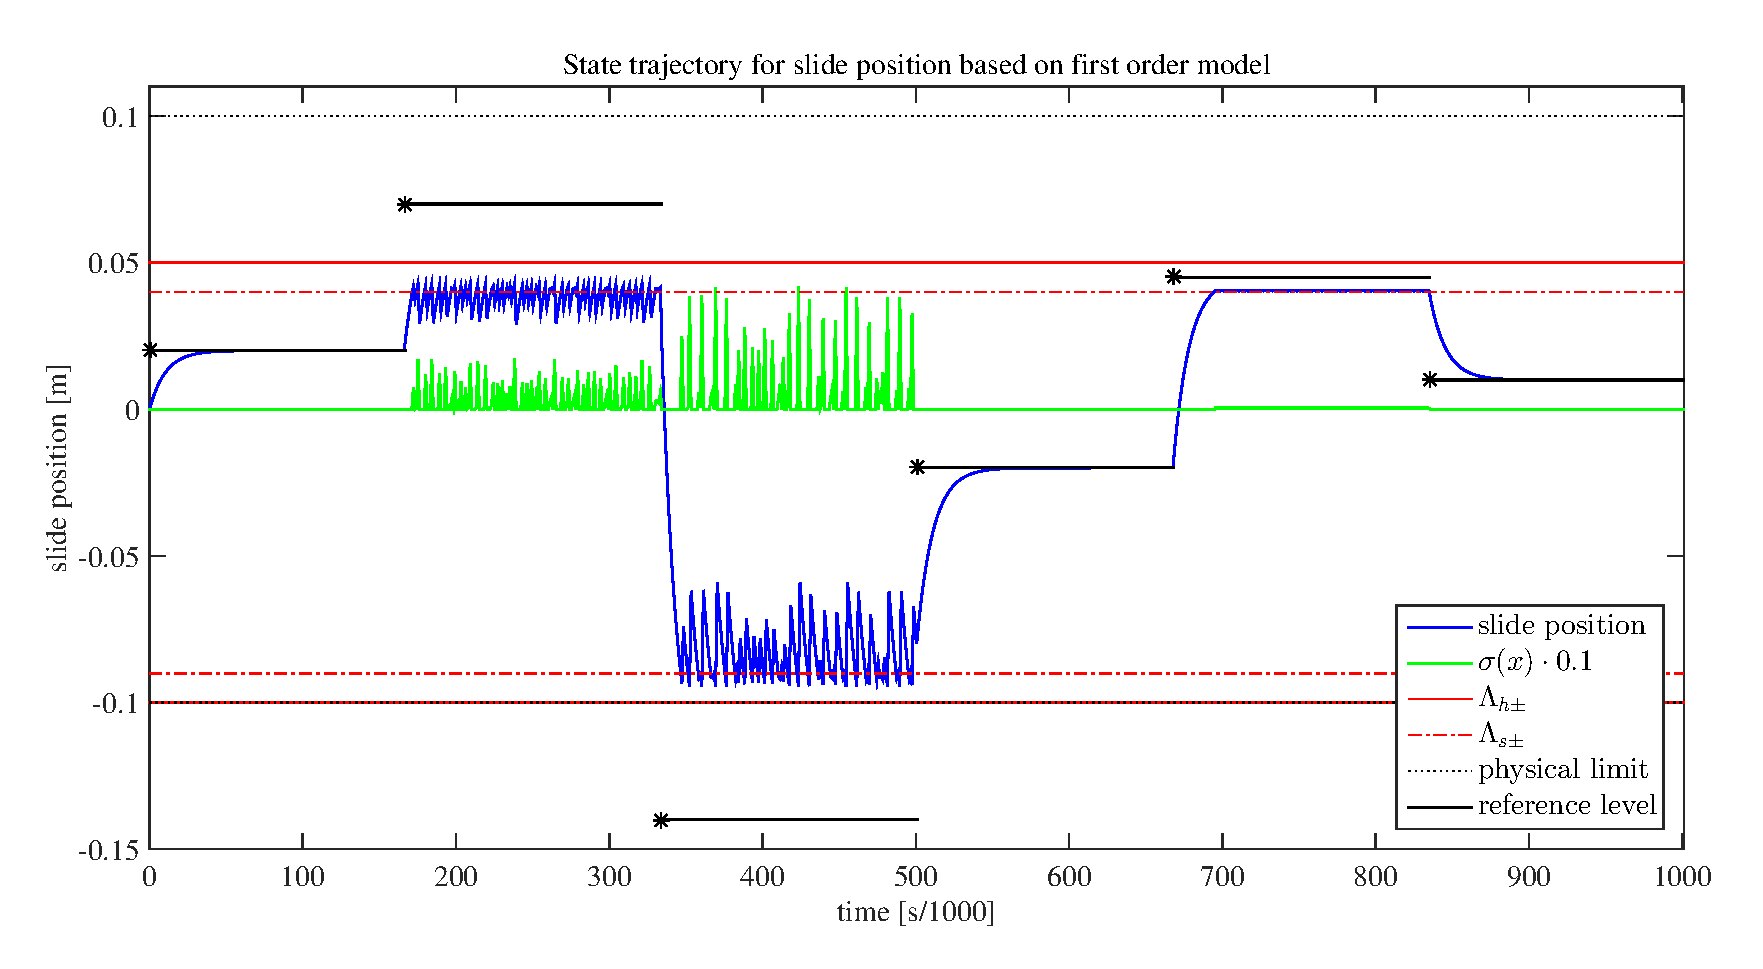
\includegraphics[scale=0.5]{trajectory_slide_kappa_10.eps}
%	\caption{State trajectory for slide position for $\kappa=10$ based on same control law and model as \autoref{fig:trajectory1}. It is seen how the safety controller is more aggressive.}
%	\label{fig:trajectory2}
%\end{figure}

To verify that \autoref{req2} is fulfilled in the simulation, the Lie derivatives are plotted in \autoref{fig:lie1}.
\begin{figure}[H]
	\center
		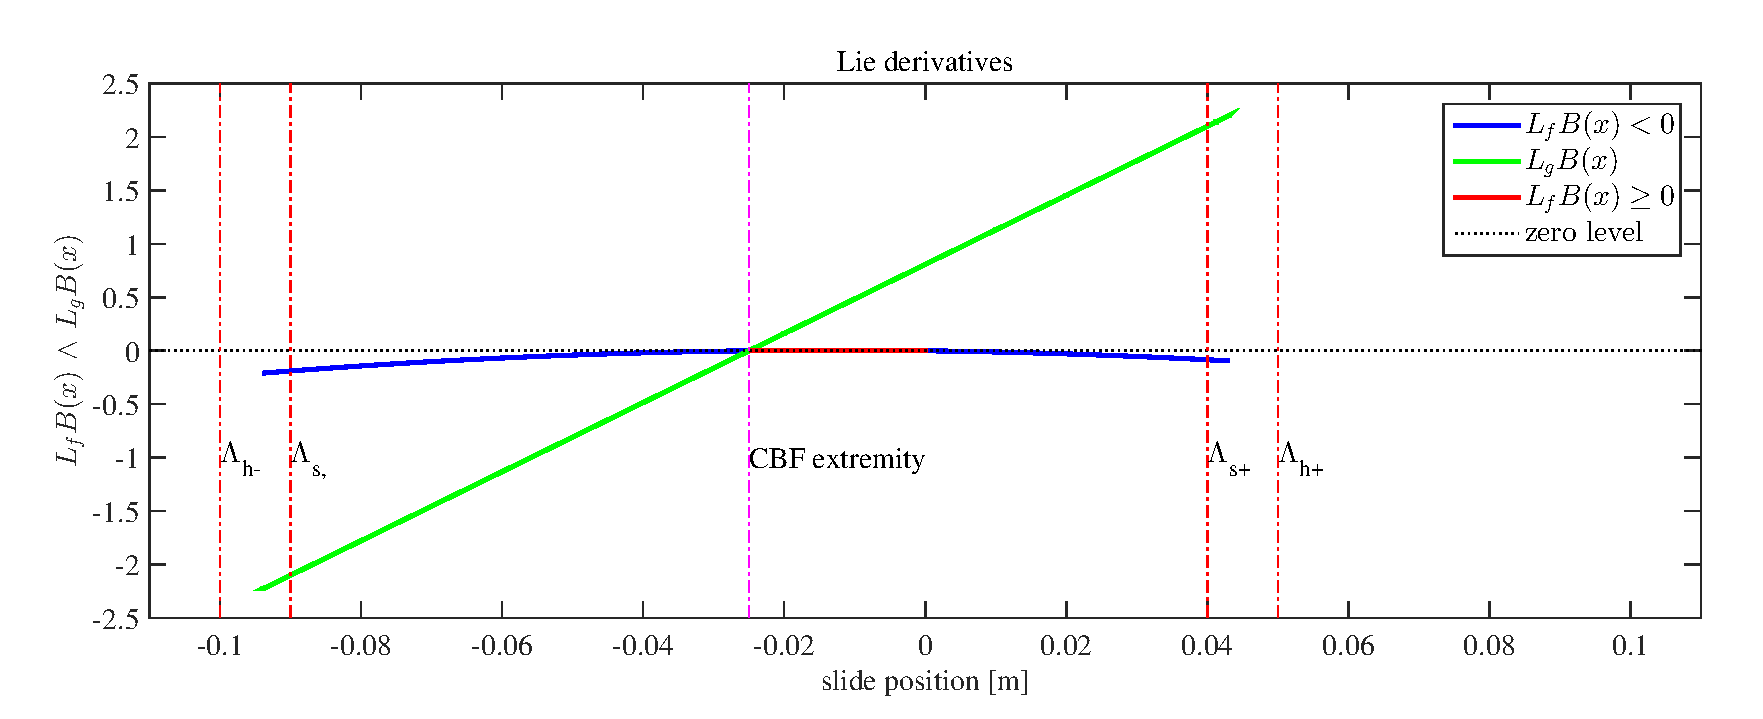
\includegraphics[scale=0.55]{Lie_slide_1d.eps}
	\caption{Lie derivatives of the CBF along the vector fields $f(x) = Ax$ and $g(x)=B$. It is seen that $L_gfB(x) \neq 0 \,\, \forall x \neq \frac{-b}{2a}$ which essentially fulfils \autoref{req2}.}
	\label{fig:lie1}
\end{figure}
It is from \autoref{fig:lie1} seen that $L_gB(x) \neq 0 \,\, \forall x \neq -b/(2a)$ which essentially fulfils \autoref{req2}. Indeed, even if the entire range $[\Lambda_{h-}:\Lambda_{h+}]$ belongs to $\mathcal{X}$, the chosen CBF would have been valid because the only place where $L_gB(x) = 0$ is at the critical point. Note also that the Lie derivatives are independent of the scalar $\kappa$.
%For the record, the control signal is plotted in \autoref{fig:control1}.
%\begin{figure}[H]
%	\center
%		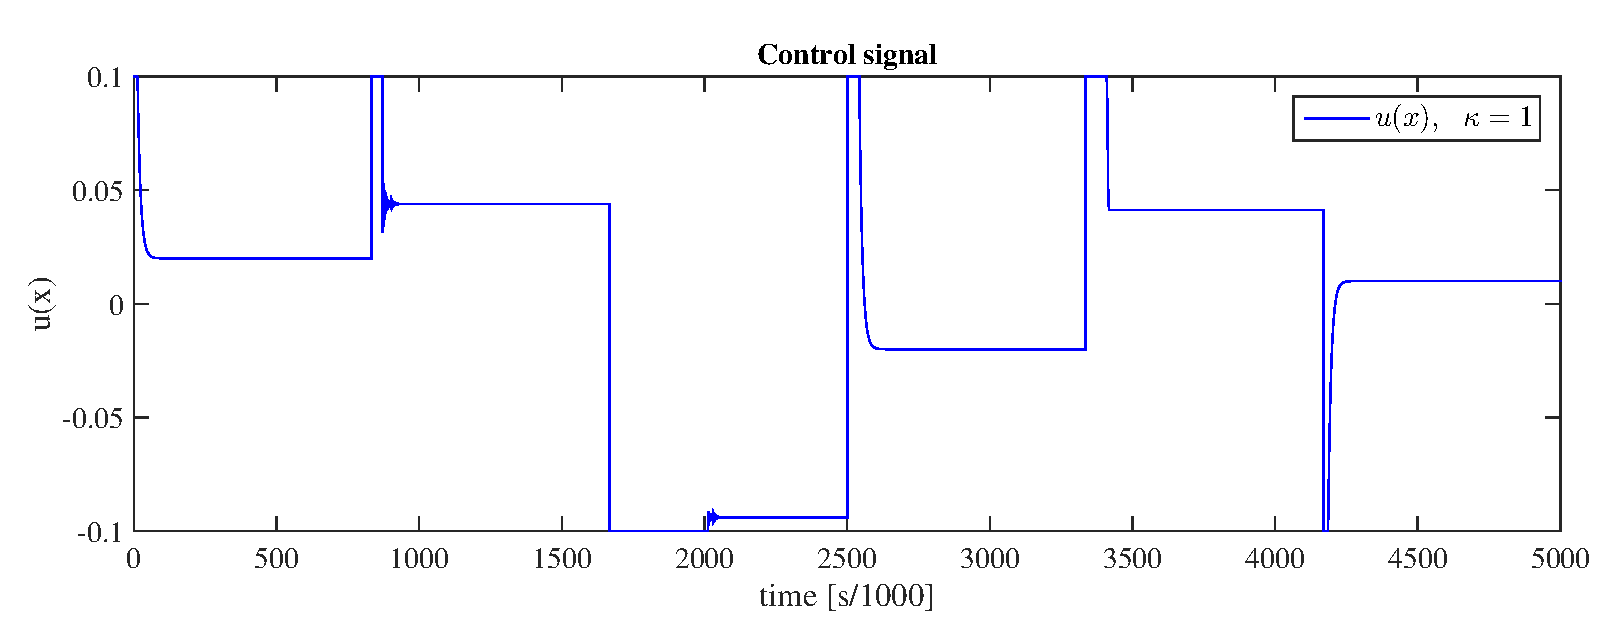
\includegraphics[scale=0.55]{control_slide_1.eps}
%	\caption{Control signal for $\kappa=1$. It is seen how the controller counteracts the large difference in setpoints given and in that way ensures safety. It is seen that when the absolute value of the setpoints are increased then $u(x)$ increases accordingly. The plot is ideal as no saturation constraints are given.}
%	\label{fig:control1}
%\end{figure}
%It is seen from \autoref{fig:control1} how the control signal reacts instantaneously and quite aggressive when $\Lambda_s$ is exceeded to counteract the large difference in setpoints given. It is also noted how the controller eventually settles smootly even when setpoints are given in the interval $[-\infty:\Lambda_{s-}]$ and $[\Lambda_{s+}:\infty]$. However, as the setpoints approaches $\pm \infty$, the sampling rate must also converge towards infinity. This is obviously not a realistic scenario as the slide movement is physically constrained.
\vspace{-0.3cm}
\subsection{MATLAB Results based on Second Order Model}\label{subsec:matlab-resutls-2-order}
\vspace{-0.2cm}
The state trajectory composing slide position based on the second order model is shown in \autoref{fig:traject2}.
\begin{figure}[H]
	\center
		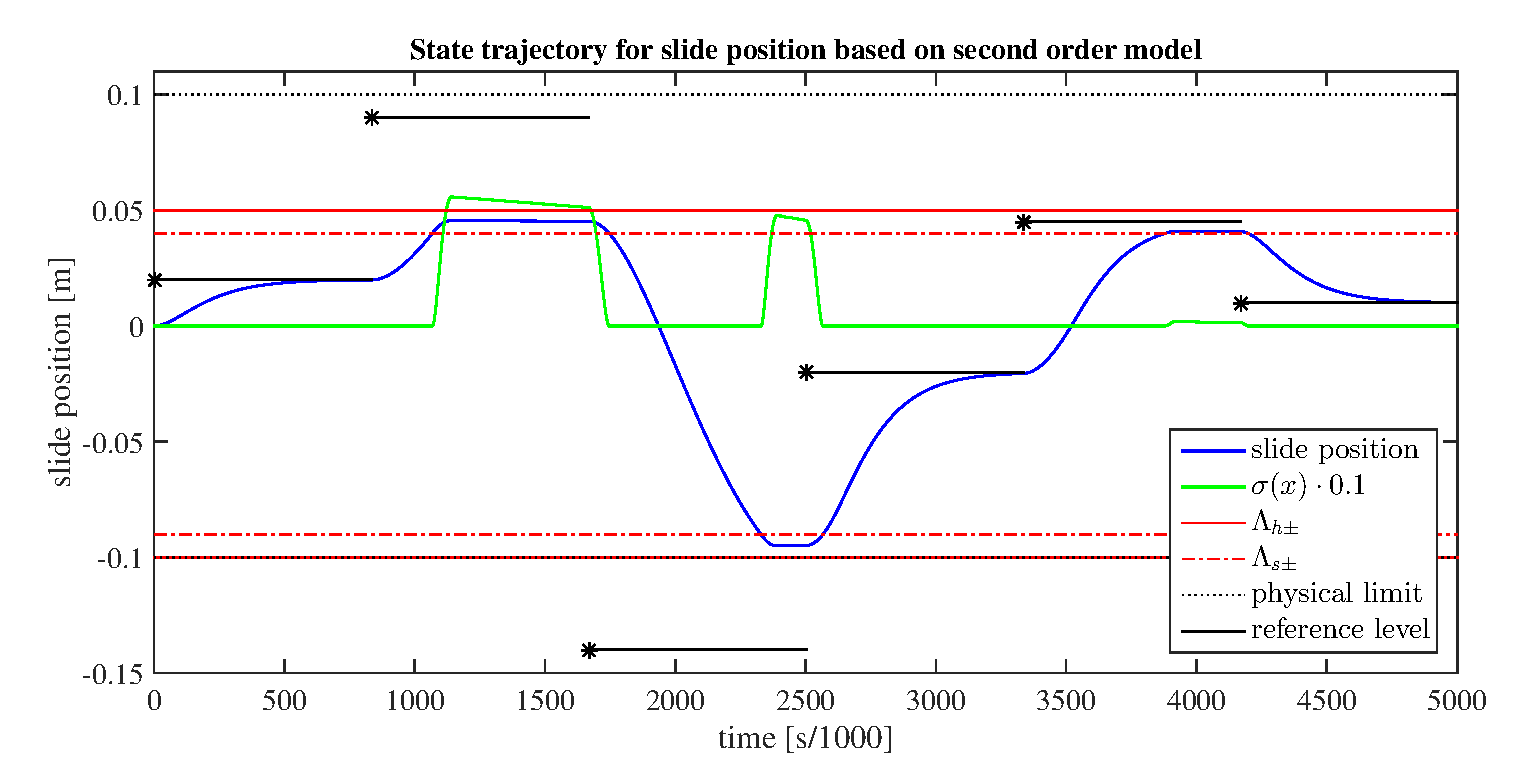
\includegraphics[scale=0.6]{trajectory_slide_second_order_model_kappa_1.eps}
	\caption{State trajectory for position based on second order system approximation. It is seen how the boundaries are respected at all time regardless of irresponsible/unsafe setpoints. It is seen how $\sigma(x)$ 	increases when setpoints are given in the unsafe area. AS a result, the control law is a linear combination of the safety controller $u(x) = k_0(x)$ and the linear controller by pole-placement $\tilde{u}(x)$.}
	\label{fig:traject2}
\end{figure}
The state trajectory shown in \autoref{fig:traject2} verifies that the slide position does not exceed its limits even when setpoints are given outside the safe region.

The Lie derivatives are plotted in \autoref{fig:lie2}.
\begin{figure}[H]
	\center
		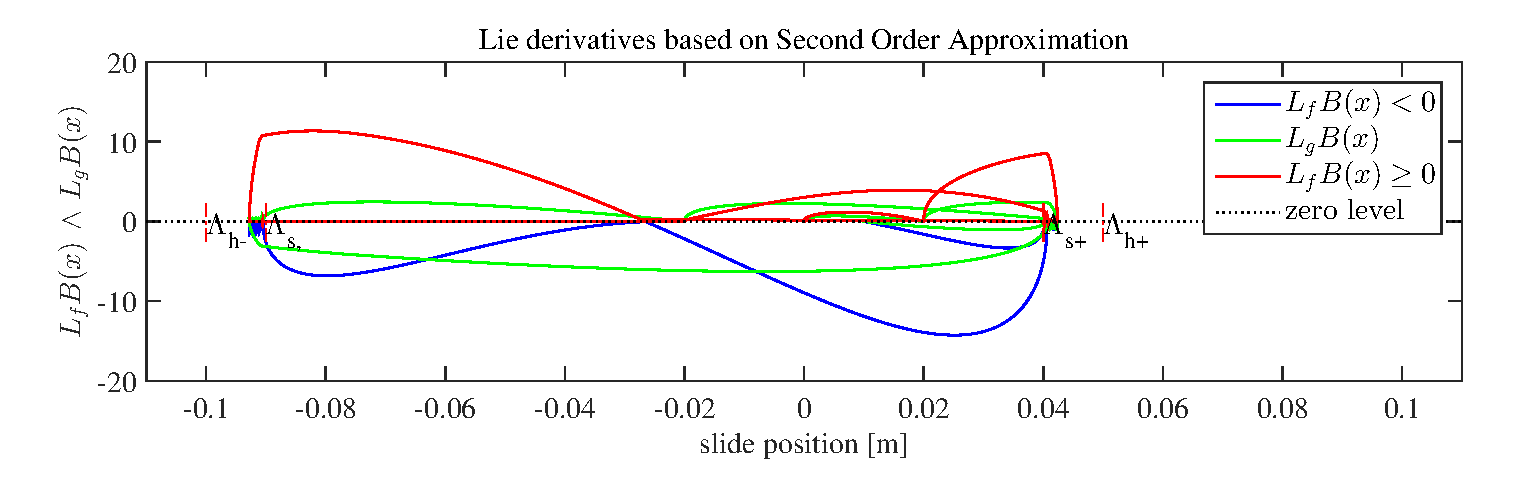
\includegraphics[scale=0.6]{Lie_slide_2d.eps}
	\caption{Lie derivatives. It is seen how $L_gB(x_1,x_2) = 0 \wedge L_fB(x_1,x_2) = 0$ at the same time which in general is critical but accepted in this specific case as it is caused by $x_2=0$ which implies $u(x)=0 \,\,\, \Rightarrow \,\,\, x_1 \rightarrow 0$ which is safe.}
	\label{fig:lie2}
\end{figure}
%The constrained control signal is plotted in \autoref{fig:control2}
%\begin{figure}[H]
%	\center
%		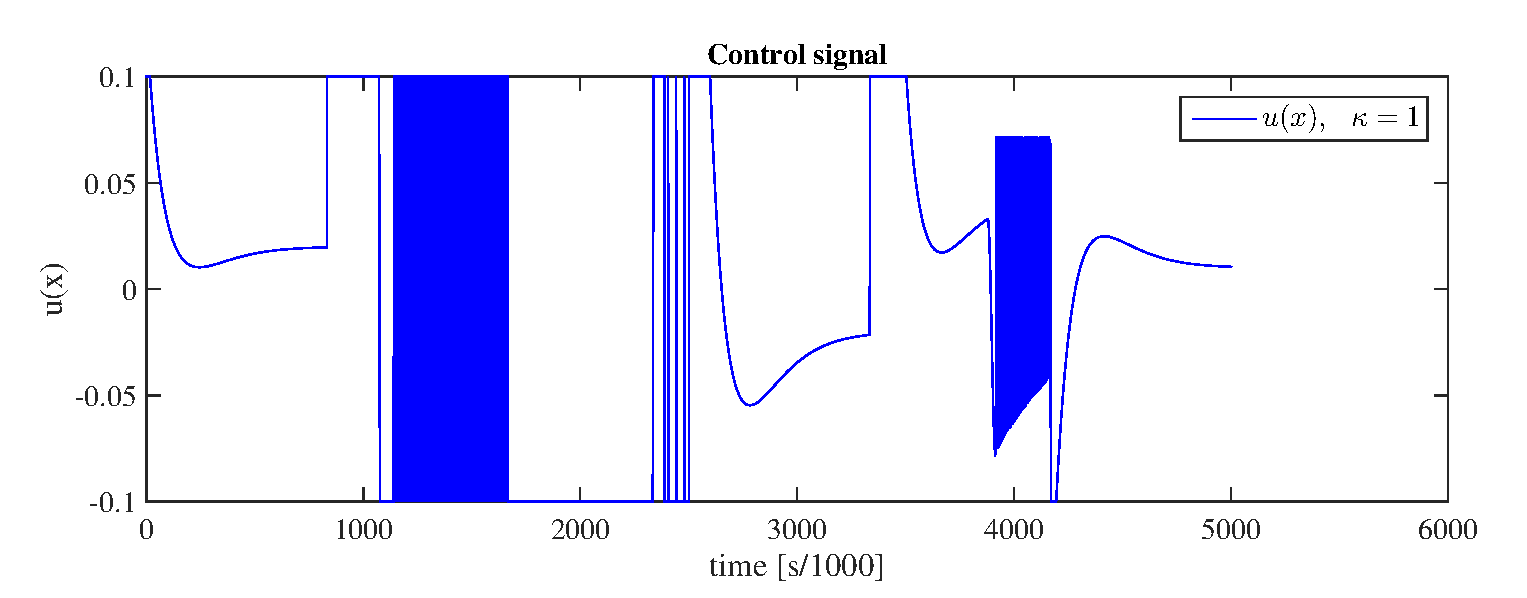
\includegraphics[scale=0.5]{control_signal_2.eps}
%	\caption{Control signal. It is seen how the it fluctuates heavily when $x_1 \in \Delta_t$ due to the position gradient.}
%	\label{fig:control2}
%\end{figure}
%It is from \autoref{fig:control2} noted how the control signal fluctuates heavily. This is because the position gradient (the velocity) changes sign constantly in the unsafe region as the trajectory seeks to go either one or the other way due to the safety controller and the setpoint given outside the safe region.

The shown plots concludes the MATLAB simulation. The MATLAB implementation shows the expected scenario, i.e. that the state trajectory complies with the outlined safe and unsafe regions.
\section{Implementation on the Da Vinci Robot}\label{sec:davinci-implementation}
The implementation constitutes the below listed bullet points:
\begin{itemize}
\item The controller will be implemented in C++. \textbf{Reason:} Along with Python, C++ is \underline{the} ROS compatible standard. The reason to use C++ over Python is to optimize speed performance. Furthermore, it is the general opinion among ROS experts (such as Postdoc Karl Damkj\ae r Hansen and others) that C++ is more useful in robot simulations and development and lastly, the already existing code at the Robotic Surgery Group - Aalborg University, is by far mostly developed in C++. However, Python as a scripting language, may be more user friendly, easier to get started with and in many cases more readable.
\item Real-time signal processing to ensure fixed sample rates. \textbf{Reason:} The observer matrices are built upon fixed sampling rates and for that reason it is crucial to comply with a fixed sample rate.
\item Algorithm development to connect these two bullet points.
\end{itemize}
The controller is implemented at the highest abstraction layer, i.e. the ROS environment depicted in \autoref{fig:overview}. While ROS runs on most Linux laptops, it is not ROS itself that put fort limitations for real time signal processing, neither is it the potentiometers that measures the angle. The bottleneck is caused by the TCP/IP communication channel which according to Assistant Engineer Simon Jensen is limited to 100\,Hz. For that reason, the maximum allowed execution time $c_{p,\text{max}}$ is:
\begin{flalign*}
c_{p,\text{max}} = \dfrac{1}{100\,\text{Hz}} = 10\,\text{ms}
\end{flalign*}
The main algorithm is depicted in \autoref{fig:slide_safery_algorithm}.
\begin{figure}[H]
	\center
		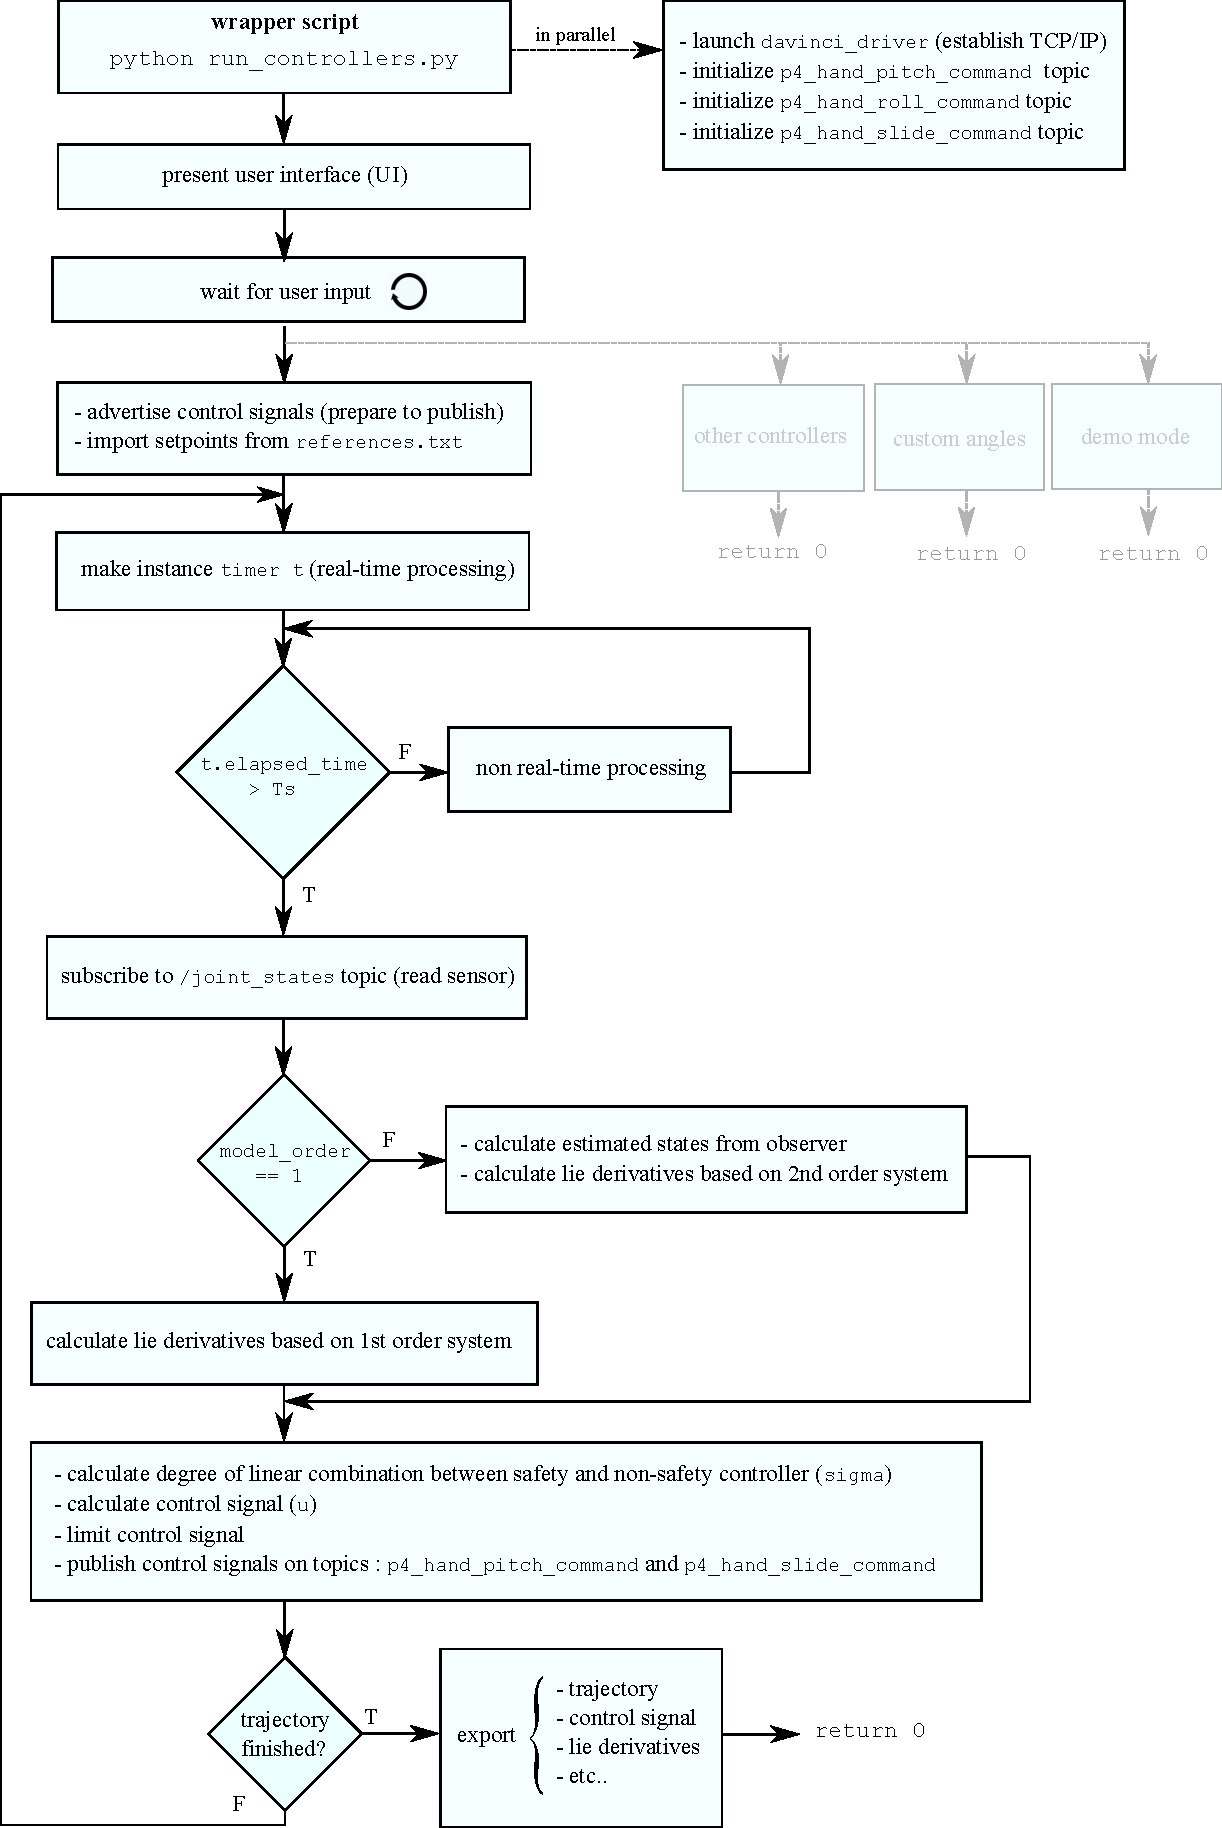
\includegraphics[scale=0.7]{flowchart_safety_controller.pdf}
	\caption{Algorithm for slide safety controller.}
	\label{fig:slide_safery_algorithm}
\end{figure}
The source code associated with the algorithm from \autoref{fig:slide_safery_algorithm} can be found in \autoref{app:slide_implement_2} and in \autoref{app:cd}. It can also be found at github at the Robotic Surgery Group - Aalborg University under the repository \texttt{gr1032} (\textit{https://github.com/AalborgUniversity-RoboticSurgeryGroup/}).
\subsection{Implementation on the Da Vinci Robot based on 1D Model}\label{subsec:implement-davinci-1d}
All plots and measurement in this subsection can be reconstructed by running the MATLAB script \texttt{plot\_data} found in \autoref{app:cd} in the folder \texttt{measurements/slide\_safety\_controller/1D\_1st\_order}. The execution time is validated first as it is essential for the controller to complete successfully. A plot measuring the execution time for each iteration is shown in \autoref{fig:exe_1}.
\begin{figure}[H]
	\center
		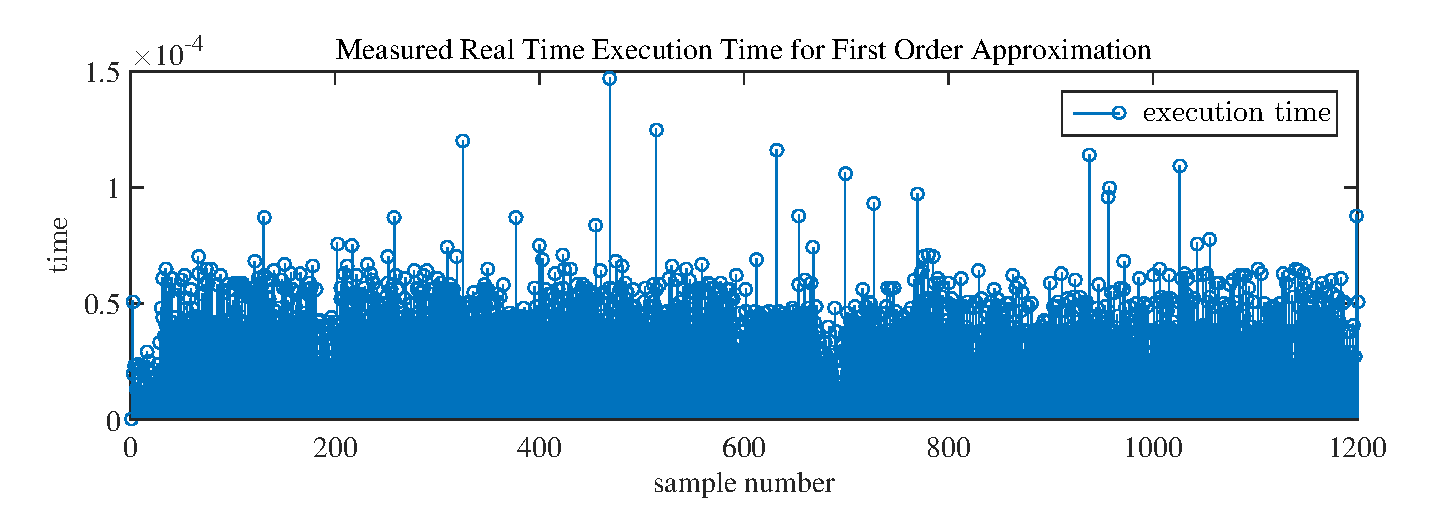
\includegraphics[scale=0.6]{execution_time_1_order.eps}
	\caption{Execution time for the first order system approximation. It is seen that the controller never exceed at computation time of 150\,$\mu$s.}
	\label{fig:exe_1}
\end{figure}
It is from \autoref{fig:exe_1} seen that $c_p < c_{p,\text{max}}$ and the real-time part is therefore verified.

The measured state trajectory is plotted in \autoref{fig:traj_meas_1}.
\begin{figure}[H]
	\center
		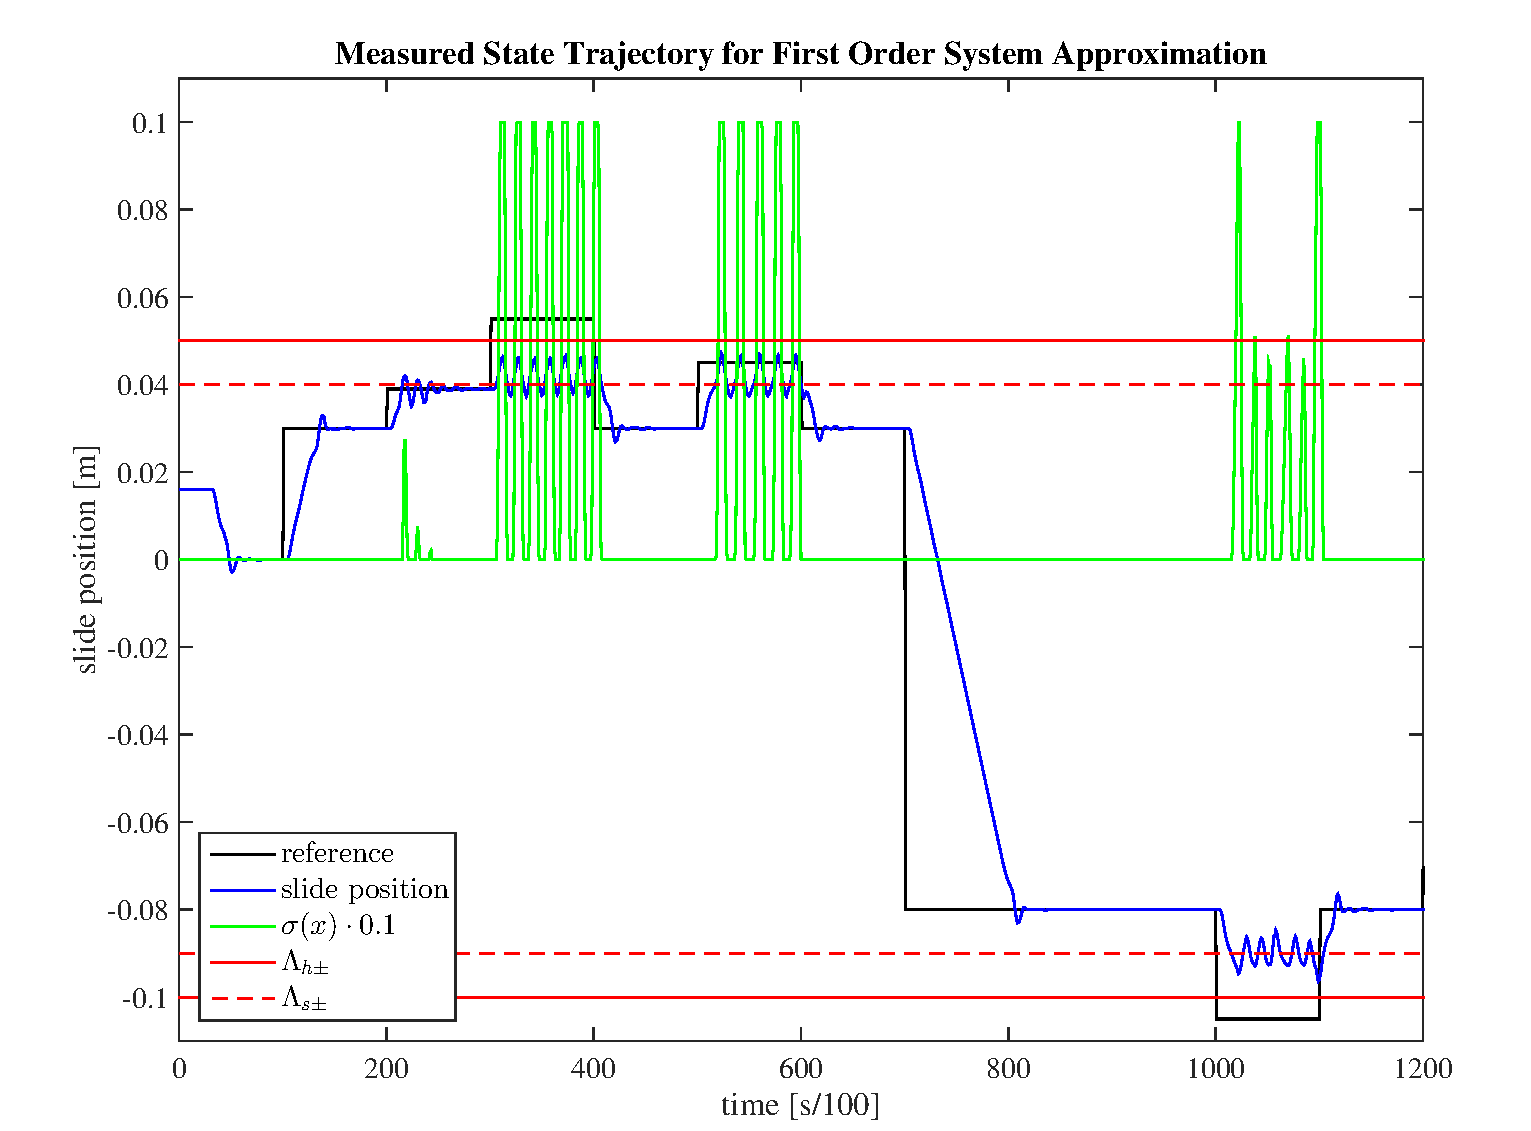
\includegraphics[scale=0.65]{trajectory_slide_meas_1.eps}
	\caption{Measured position trajectory based on the first order approximation.}
    \label{fig:traj_meas_1}
\end{figure}
It is from \autoref{fig:traj_meas_1} seen how the controller ensures that $x \in \mathcal{X}_u^c \ \ \forall \, x$. The poor system approximation is also revealed as the trajectory has an overshoot which was not included in the simulation found in \autoref{fig:trajectory1}. This is however not surprisingly as the first order approximation was created to simplify the control barrier function and to avoid the observer design as an initial approach. A consequence of the overshoot is seen when setpoints very close to $\Lambda_{s+}$ are given. The slide movement starts to oscillate which is caused by $\sigma(x)$. This is obviously not a good thing, but nevertheless the intended outcome when $x \in \mathcal{T}$. Additionally, it is seen how $\sigma(x)$ forces the position below its setpoint when $x_\text{ref} \in \mathcal{X}_u$ but allows $x_1 > x_\text{ref}$ when $x \in \mathcal{T}$. This is indeed the effect of $\sigma(x)$. It is finally seen that the safety controller is fully functional for both $\mathbb{R}^-$ and $\mathbb{R}^+$.

The Lie derivatives are calculated based on the measured position. The result is seen in \autoref{fig:meas_lie_1}
\begin{figure}[H]
	\center
		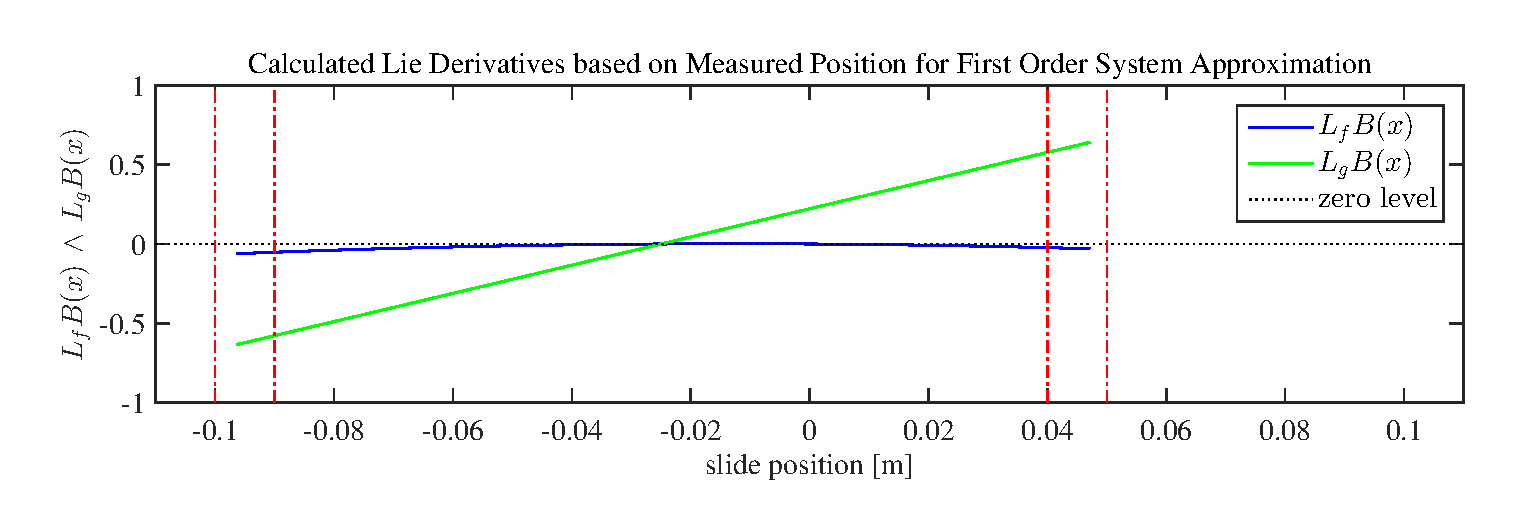
\includegraphics[scale=0.65]{meas_lie_1.eps}
	\caption{Calculated Lie derivatives based on measured position for the first order system approximation. }
    \label{fig:meas_lie_1}
\end{figure}
It is seen that the Lie derivatives from \autoref{fig:meas_lie_1} are very similar to the theoretical lie derivatives from \autoref{fig:lie1}.
%%%%%%%%%%%%
%%%%%%%%%%%%
%%%%%%%%%%%%
%%%%%%%%%%%%
\subsection{Implementation on the Da Vinci Robot based on 2D Model}\label{subsec-implement-2dmodel}
All plots and measurement in this subsection can be reconstructed by running the MATLAB script \texttt{plot\_data} found in \autoref{app:cd} in the folder \texttt{measurements/slide\_safety\_controller/2D\_2nd\_order}. Again, the execution time is validated first. A plot measuring the execution time for each iteration is shown in \autoref{fig:exe_1}.
\begin{figure}[H]
	\center
		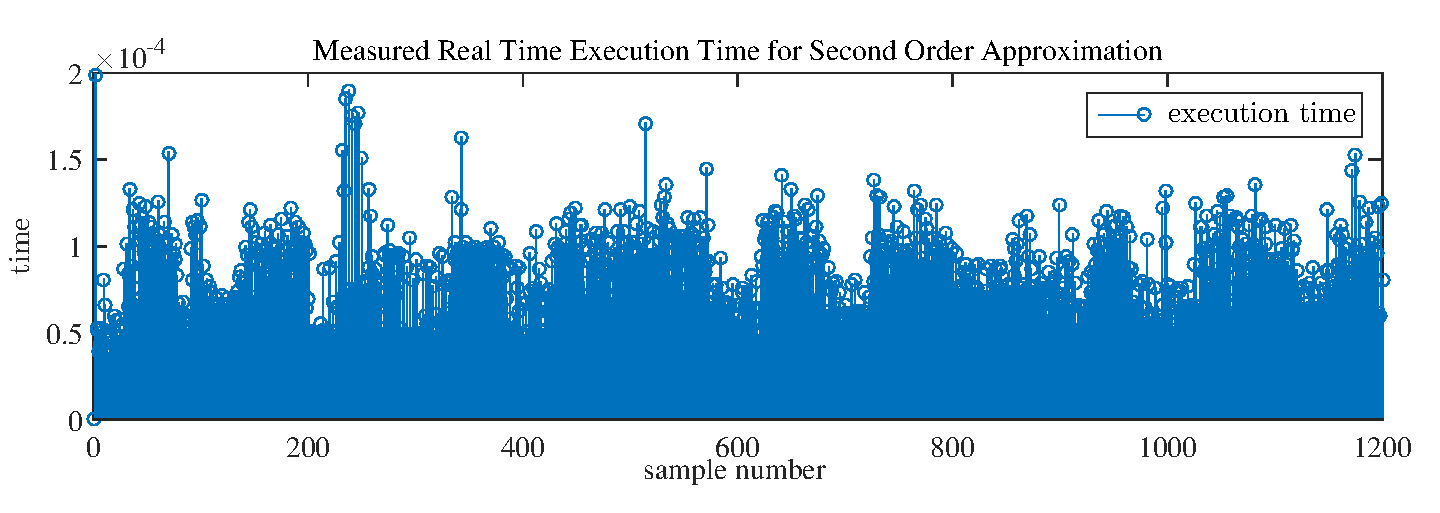
\includegraphics[scale=0.6]{execution_time_2_order.eps}
	\caption{Execution time for second order system approximation. It is seen that the controller never exceed at computation time of 200\,$\mu$s.}
	\label{fig:exe_2}
\end{figure}
It is from \autoref{fig:exe_2} seen that the real time part is completed within the allowed 10\,ms (100\,Hz). Note that the execution time is slightly higher than in \autoref{fig:exe_1} because the velocity is estimated with the observer.

The measured state trajectory is plotted in \autoref{fig:traj_meas_1}.
\begin{figure}[H]
	\center
		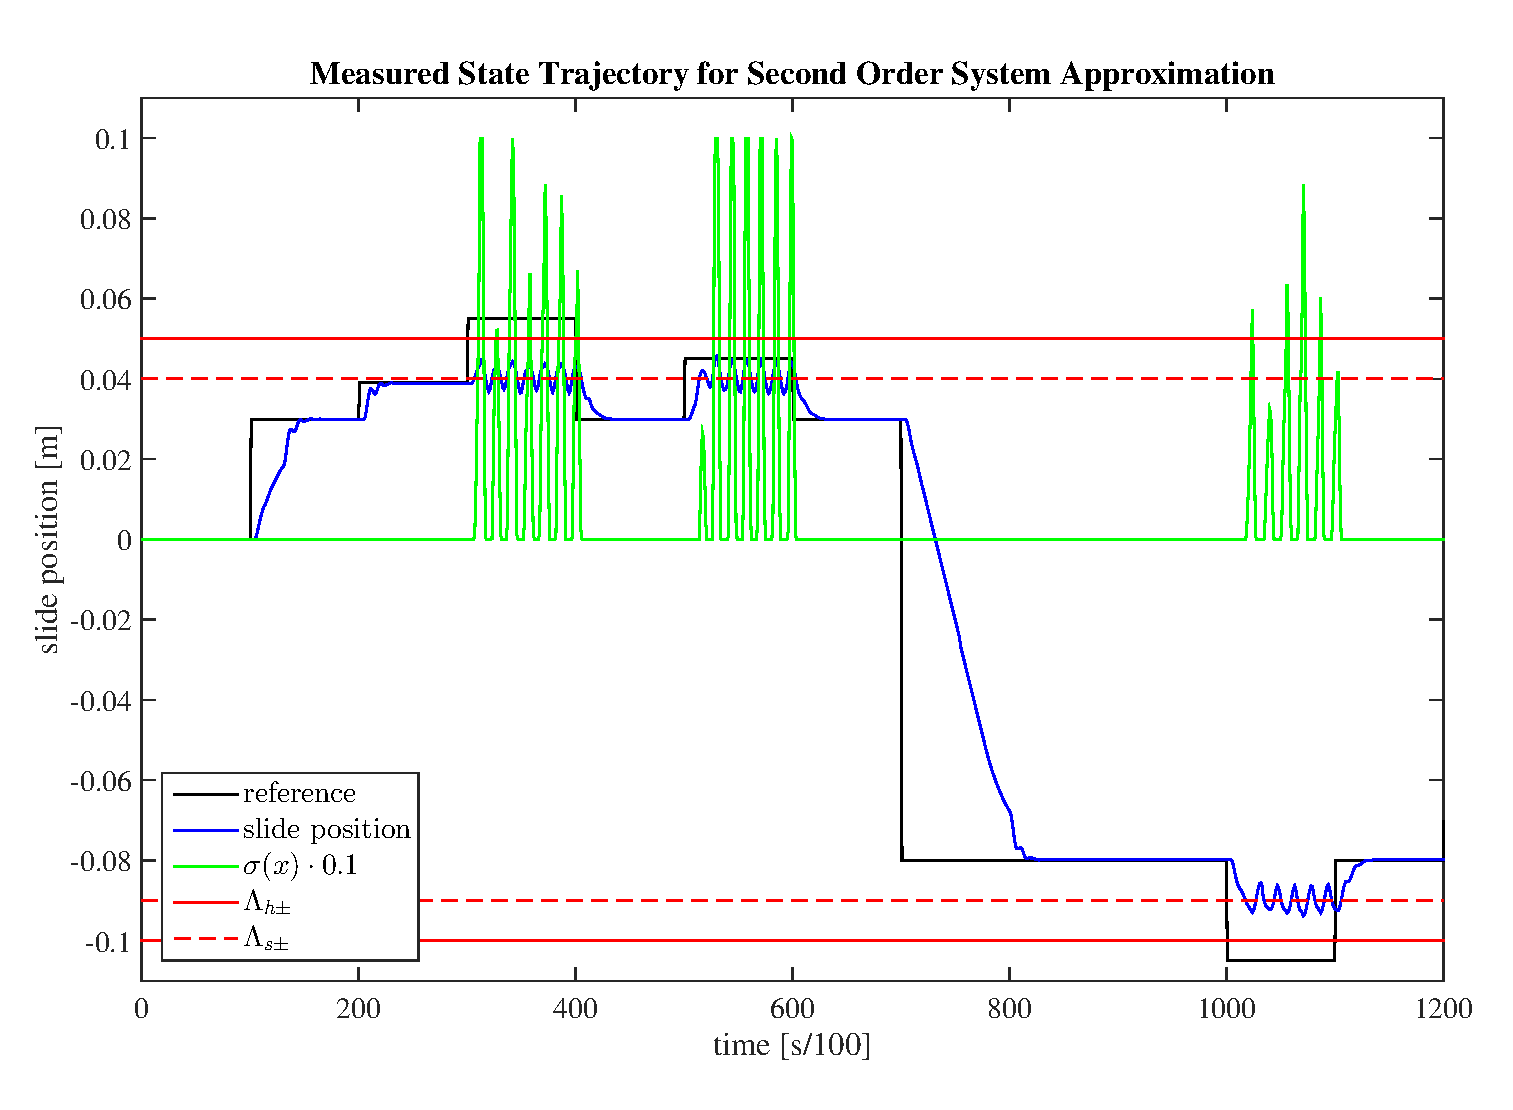
\includegraphics[scale=0.65]{meas_trajectory_2_order.eps}
	\caption{Measured position trajectory based on the second order approximation.}
    \label{fig:traj_meas_2}
\end{figure}
It is from \autoref{fig:traj_meas_2} seen how the overshoot is eliminated. This was indeed the main purpose of the development of a controller based on a second order approximation. Also, note how it is possible to give setpoints close to the the set $\mathcal{T}$ and still avoid oscillations caused by $\sigma(x)\neq 0$. This is a big advantage when a doctor needs to operate close to an unsafe regions. Finally, just as in \autoref{fig:traj_meas_1}, it is seen how $\sigma(x)$ forces the position below its setpoint when $x_\text{ref} \in \mathcal{X}_u$ but allows $x_1 > x_\text{ref}$ when $x \in \mathcal{T}$. This is indeed the effect of $\sigma(x)$.

The Lie derivatives are calculated based on the measured position and the estimated velocity. The result is seen in \autoref{fig:meas_lie_2}
\begin{figure}[H]
	\center
		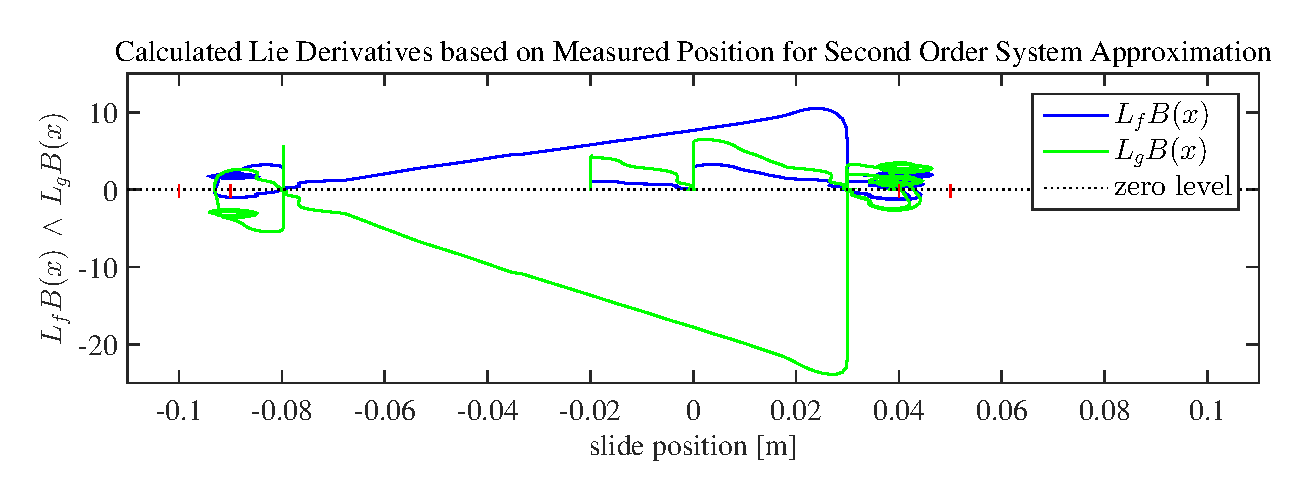
\includegraphics[scale=0.65]{meas_lie_2.eps}
	\caption{Calculated Lie derivatives based on measured position and estimated velocity for the second order system approximation. }
    \label{fig:meas_lie_2}
\end{figure}
It is seen that the Lie derivatives from \autoref{fig:meas_lie_2} are quite different that from \autoref{fig:lie2}. This is due to an imprecise estimation of the estimated velocity.
\subsection{Conclusion for Slide Safety Controller}\label{subsec:conclusion-slide-safety}

